\chapter{Implementation - Tool}
This project has been implemented as an MITK plugin. MITK, the Medical Imaging Interaction Toolkit, is a free open-source software system for the development of interactive medical image processing software. It combines ITK (for image processing) and VTK (for visualization) together and provides a basic application, the MITK Workbench, that can be extended with plugins.

\begin{figure}[H]
  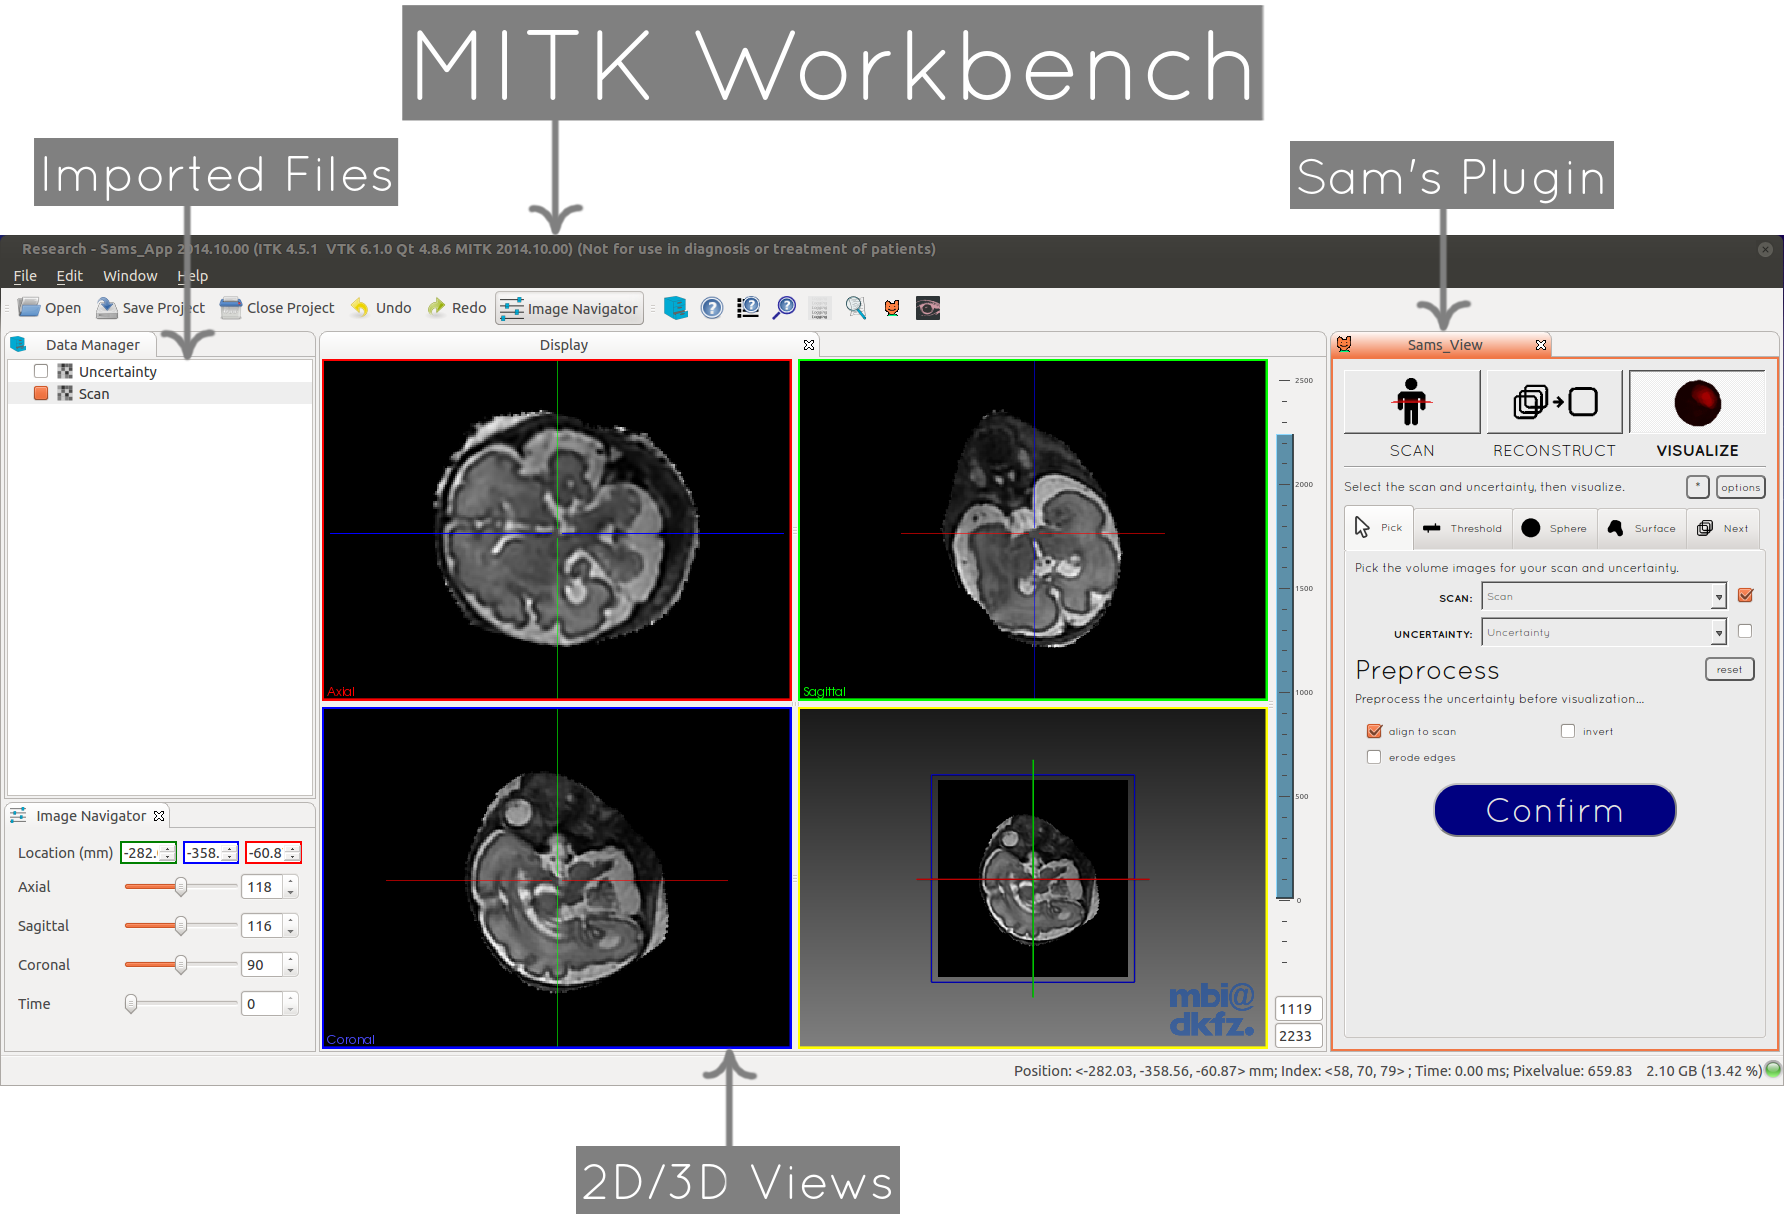
\includegraphics[width=\textwidth]{images/tool/mitk.png}
  \caption{MITK Workbench + Plugin}\label{fig:scansettings}
\end{figure}

The plugin that has been developed is a research prototype designed primarily to visualize the uncertainty in MRI reconstructions. However, it also begins to integrate all parts of the reconstruction pipeline together into one application. Broadly speaking the pipeline can be split into three steps: scan -> reconstruct -> visualize. The plugin developed incorporates components from each stage.

\subsection*{Scan Simulation}
Given a previous reconstruction, that is assumed to be a perfect, ground truth, representation, we can simulate a scan by re-sampling it.

\subsection*{Reconstruct}
Using slice stacks (simulated or otherwise) we can reconstruct a super resolution image. Optionally landmarks can be provided to guide the registration process.

\subsection*{Visualize}
When the reconstruction has finished we can visualize how well it went.
\begin{itemize}
  \item Thresholding
  \item Uncertainty Sphere
  \item Uncertainty Surface
  \item Next Scan Plane
\end{itemize}

\newpage
\section{Scan Simulation}\label{section:simulatescan}
The idea behind simulating a scan is that we can evaluate the performance of reconstruction algorithms if we can compare the result to a known, 'perfect', reconstruction. This idea was used in the same paper concerned with finding the optimum scan plane\cite{uncertaintysvd}. The focus of this part of the tool is not to evaluate the effectiveness of this approach, that is a project in it's own right, but to make this simulation easier to perform and customize for future research.

\begin{wrapfigure}[23]{r}{0.4\textwidth}
  \vspace{-20pt}
  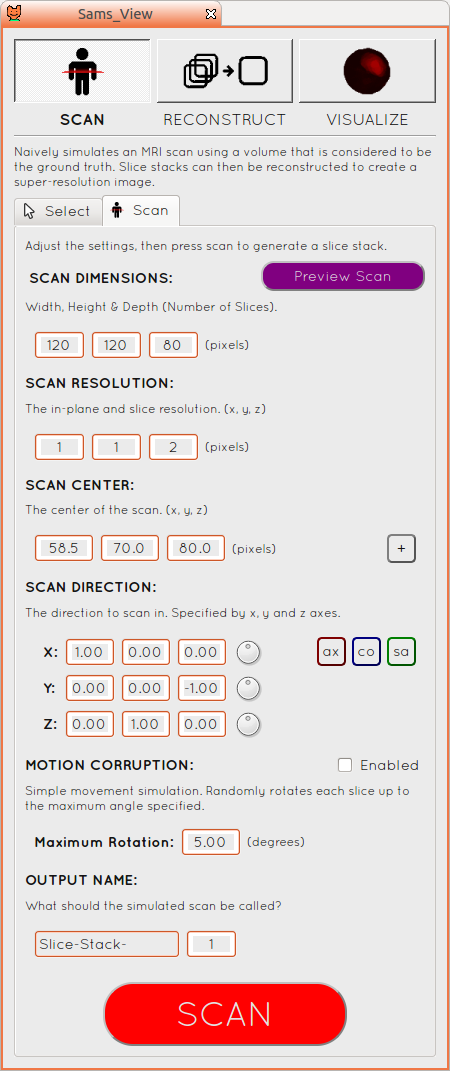
\includegraphics[width=0.4\textwidth]{images/scan_simulation/scan_settings.png}
  \caption{Controls}\label{fig:scansettings}
\end{wrapfigure}

The user has a number of controls (see figure \ref{fig:scansettings}) available to tweak:

\subsection*{Scan Dimensions}
Number of pixels in the scan (x, y, z).

\subsection*{Scan Resolution}
Size of each pixel, relative to the reconstructed scan (x, y, z).

\subsection*{Scan Center}
The center point of the scan (x, y, z). This can be set to the center of the volume or adjusted manually.

\subsection*{Scan Direction}
The direction to scan in. You may expect this to be just one vector (the z-direction) but since the scan is rectangular in shape the x and y-direction also need to be specified. The standard axial, coronal and sagittal directions are available and the direction can be rotated about each axis using the dials.

\subsection*{Motion Corruption}
Some simple motion corruption can be enabled. Currently the implementation is quite simple; the motion only happens in between slices being scanned. Before each slice gets scanned a random rotation (up to a maximum specified) is applied about a random axis to the original image.

Figure \ref{fig:scansimulationexample} shows an example of an axial scan (y-axis) where the preview is overlayed on a volume rendering of the ground truth volume. The preview box shows the boundary of the scan, which is updated to show any changes to the configuration. The effects of the motion corruption are apparent when viewed from the side; successive stacks don't line up.

\begin{figure}[H]
  \centering
  \begin{subfigure}[b]{0.5\textwidth}
    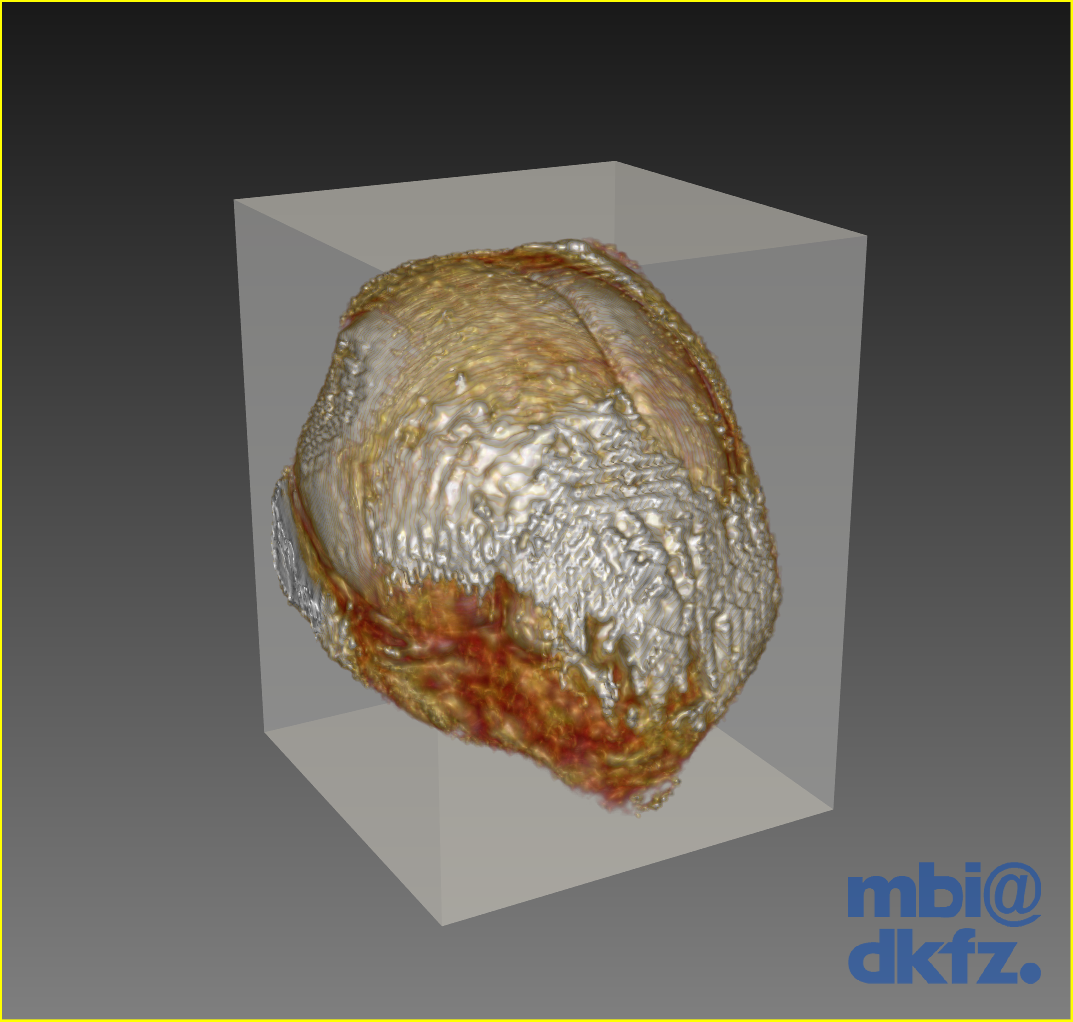
\includegraphics[width=\textwidth]{images/scan_simulation/scan_axial_preview.png}
    \caption{Axial Scan Preview}\label{fig:scansimulationpreview}
  \end{subfigure}%
  ~ %add desired spacing between images, e. g. ~, \quad, \qquad, \hfill etc.
    %(or a blank line to force the subfigure onto a new line)
  \begin{subfigure}[b]{0.5\textwidth}
    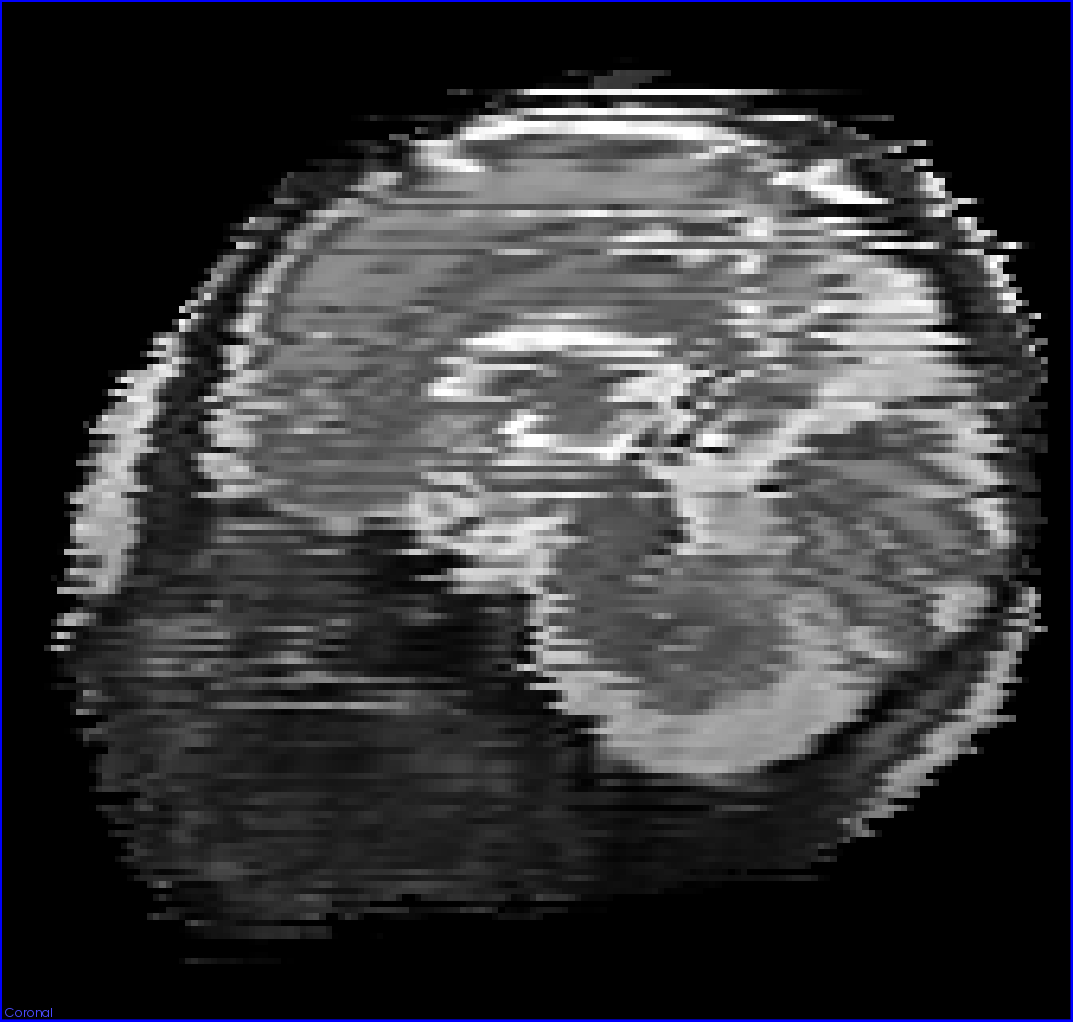
\includegraphics[width=\textwidth]{images/scan_simulation/scan_axial_result.png}
    \caption{Side (Sagittal) View of Simulation}\label{fig:scansimulationresult}
  \end{subfigure}
  \caption{Example Scan Simulation.}\label{fig:scansimulationexample}
\end{figure}

\newpage
\section{Reconstruction}\label{section:reconstruction}
This part of the tool uses the fast GPU reconstruction code developed in \cite{uncertaintysvd}. The Common Toolkit (CTK) includes functionality that allows you to run external binaries from within MITK\cite{ctkcmd}. A wrapper executable has been written, which conforms to the Command Line Module XML Schema, which essentially allows the MITK plugin to make calls to the GPU reconstruction code and automatically import the result.

One of the ways that the quality of the reconstruction can be improved is by manually labelling landmarks in the scans, such as the eyes and extreme points of the skull. This helps the registration step of the reconstruction align each of the initial scans. A prototype to allow each stack to be marked up in this way has been developed with the view of getting the opinion of researchers on whether this is a process they are willing to do, or even if they have the time to do it.

Figure \ref{fig:reconstructionlandmarks} shows the process with some example landmarks. Each landmark can be placed, moved, deleted and you can also jump quickly to a previously marked point.

\begin{figure}[H]
  \centering
  \begin{subfigure}[b]{0.358\textwidth}
    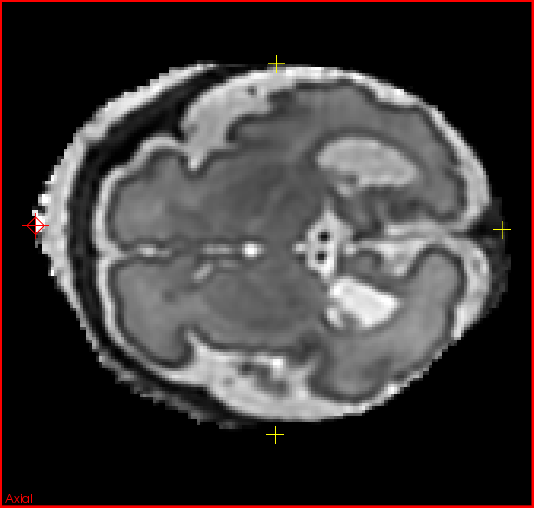
\includegraphics[width=\textwidth]{images/reconstruction/axial.png}
    \caption*{Axial}
    \label{fig:reconstructionaxial}
  \end{subfigure}%
    %add desired spacing between images, e. g. ~, \quad, \qquad, \hfill etc.
    %(or a blank line to force the subfigure onto a new line)
  \begin{subfigure}[b]{0.358\textwidth}
    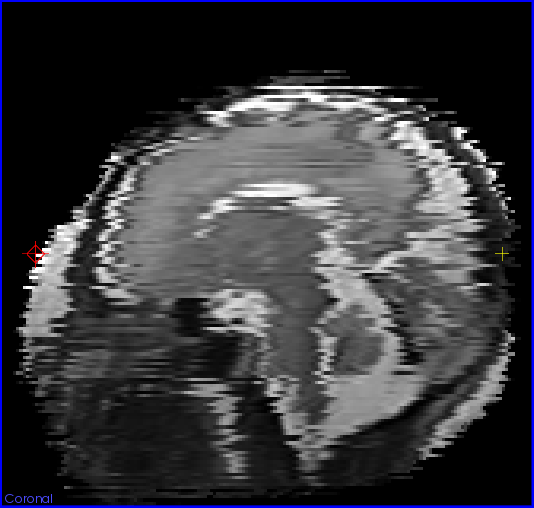
\includegraphics[width=\textwidth]{images/reconstruction/sagittal.png}
    \caption*{Sagittal}
    \label{fig:reconstructionsagittal}
  \end{subfigure}%
    %add desired spacing between images, e. g. ~, \quad, \qquad, \hfill etc.
    %(or a blank line to force the subfigure onto a new line)
  \begin{subfigure}[b]{0.283\textwidth}
    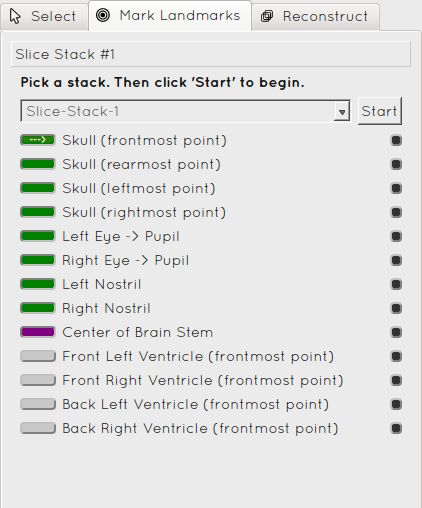
\includegraphics[width=\textwidth]{images/reconstruction/controls.png}
    \caption*{Controls}
    \label{fig:reconstructioncontrols}
  \end{subfigure}
  \caption{Placing Landmarks on Slice Stacks.}\label{fig:reconstructionlandmarks}
\end{figure}

\newpage
\chapter{Implementation - Visualizations}\label{sectiontoolvisualization}
This is where the visualizations live. The demo ones are available.

Show screenshot (annotated).
\begin{figure}[h]
  \centering
  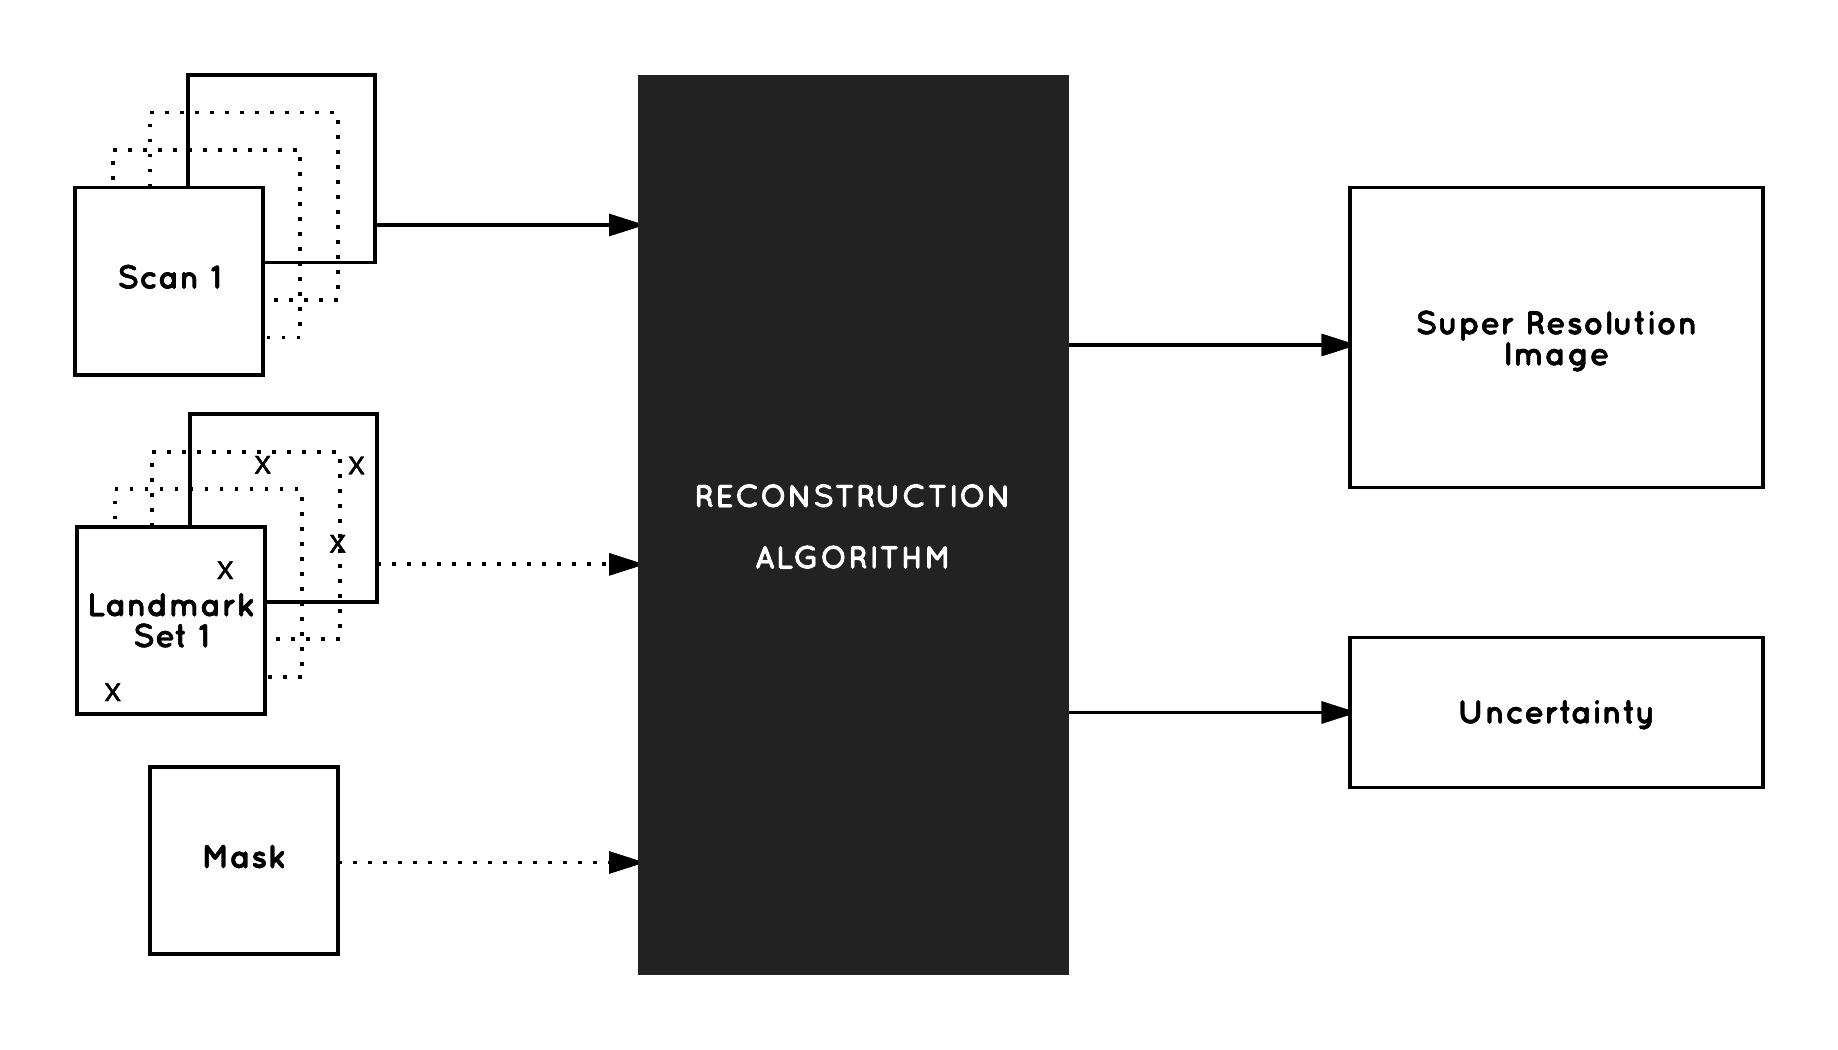
\includegraphics[width=0.8\textwidth]{images/reconstruction_overview.png}
  \caption{Reconstruction Overview}
  \label{fig:erosionbefore}
\end{figure}

The super resolution reconstruction process takes in a set of slice stacks (scans), an optional mask and outputs the reconstructed MRI volume and the uncertainty. The mask is used to ignore areas that are not of interest; for example when doing a fetal scan a mask can be created to ignore surrounding areas like the womb and amniotic fluid.

\section{Preprocessing}\label{section:preprocessing}
The uncertainty tells us for each pixel in the reconstructed volume how much confidence we have in that value. However, before we can visualize it some preprocessing must be applied. 

\subsection*{Normalization}
The uncertainty is linearly scaled so each value is between 0 and 1.

\begin{verbatim}
  0 - no information (high uncertainty - worst)
  1 - maximum information (low uncertainty - best)
\end{verbatim}

\subsection*{Erosion}
The optional erosion step removes the uncertainty values at the edge of the reconstruction. The edges often have a much higher uncertainty either because there are fewer slices to use or the mask cuts off the data required. Removing this edge helps the visualization to focus on the core of the volume.

The edges are removed in five steps:

\begin{enumerate}
  \item An erosion filter is applied to the image. This removes the edges but has the unwanted effect of also eroding uncertainty in the center of the volume.
  \item The absolute difference is taken between the original and the eroded image.
  \item The difference is then thresholded to create a mask of the areas that changed the most. The idea here is that the edges change significantly more than the small pockets of uncertainty inside.
  \item A growing filter is applied to the mask, to ensure the entire edge is covered.
  \item Finally all the points in the mask are set to 0 to remove the edge.
\end{enumerate}

Figure \ref{fig:erosionoverview} shows how the soft fade out of uncertainty due to the mask is removed to create a hard edge.

\begin{figure}[h]
  \centering
  \begin{subfigure}[b]{0.3\textwidth}
    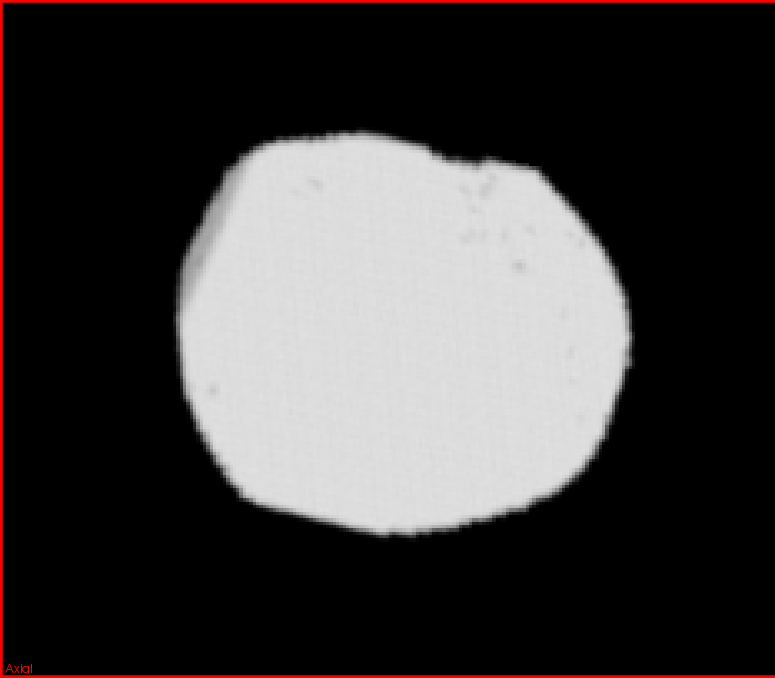
\includegraphics[width=\textwidth]{images/erosion/erosion_0.png}
    \caption{Original}
    \label{fig:erosion0}
  \end{subfigure}%
  ~ %add desired spacing between images, e. g. ~, \quad, \qquad, \hfill etc.
    %(or a blank line to force the subfigure onto a new line)
  \begin{subfigure}[b]{0.3\textwidth}
    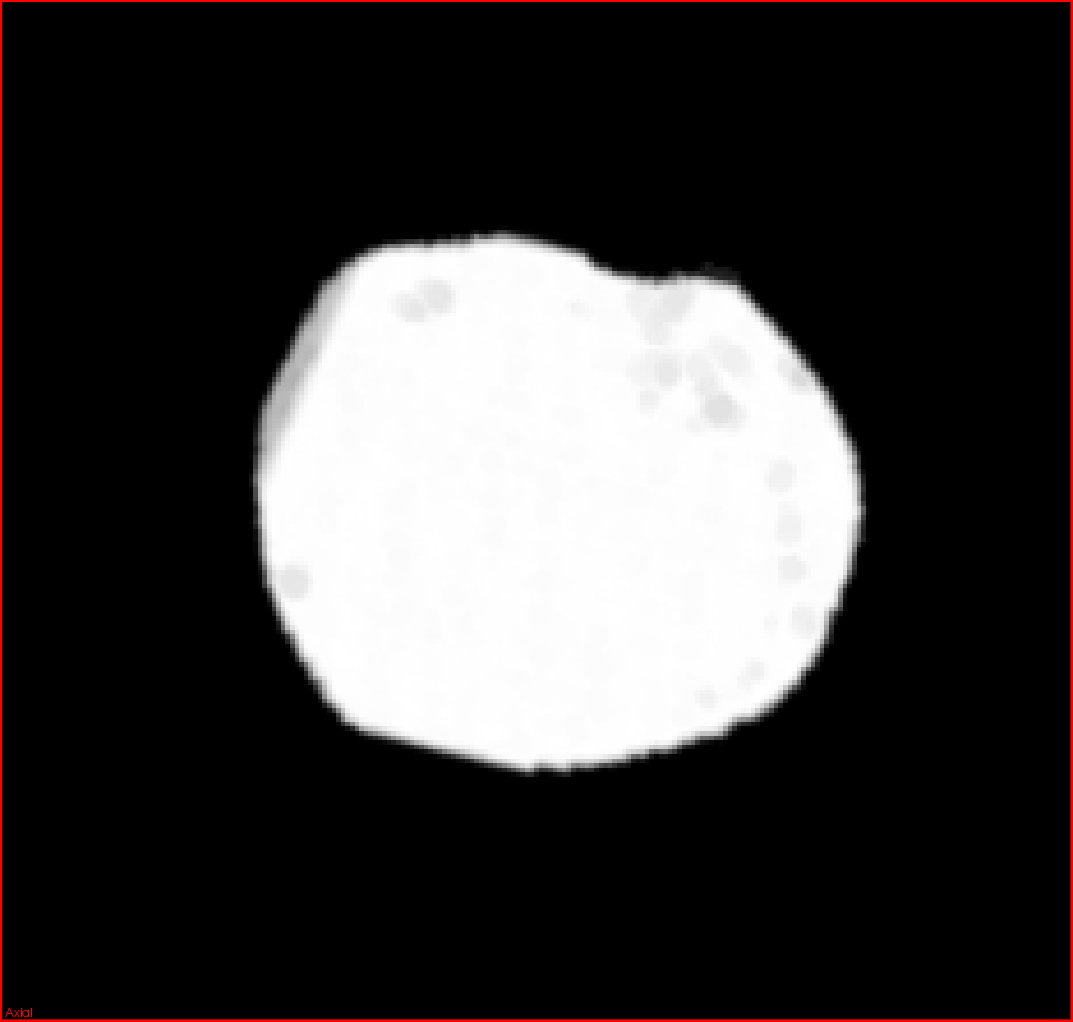
\includegraphics[width=\textwidth]{images/erosion/erosion_1.png}
    \caption{Step 1}
    \label{fig:erosion1}
  \end{subfigure}  
  ~ %add desired spacing between images, e. g. ~, \quad, \qquad, \hfill etc.
    %(or a blank line to force the subfigure onto a new line)
  \begin{subfigure}[b]{0.3\textwidth}
    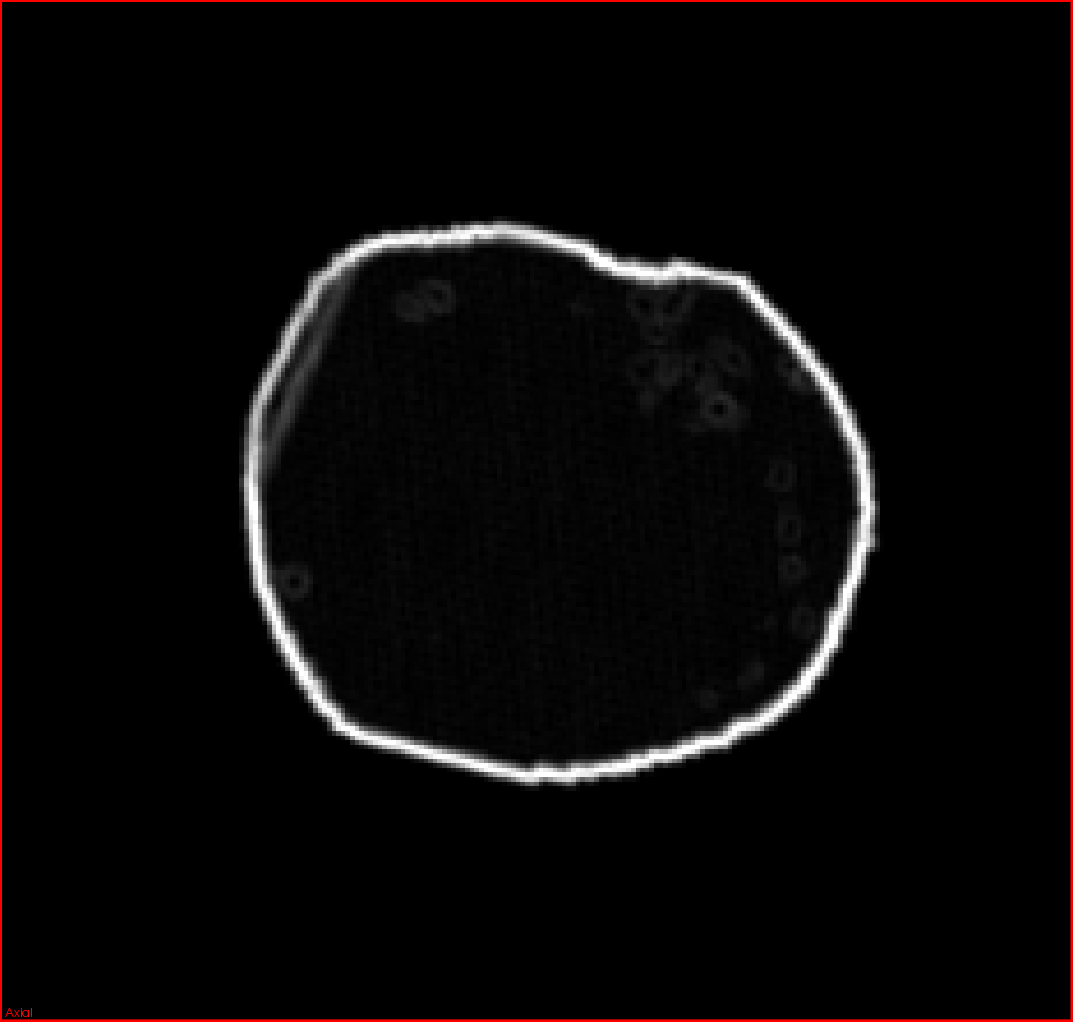
\includegraphics[width=\textwidth]{images/erosion/erosion_2.png}
    \caption{Step 2}
    \label{fig:erosion2}
  \end{subfigure}
  ~ %add desired spacing between images, e. g. ~, \quad, \qquad, \hfill etc.
    %(or a blank line to force the subfigure onto a new line)
  \begin{subfigure}[b]{0.3\textwidth}
    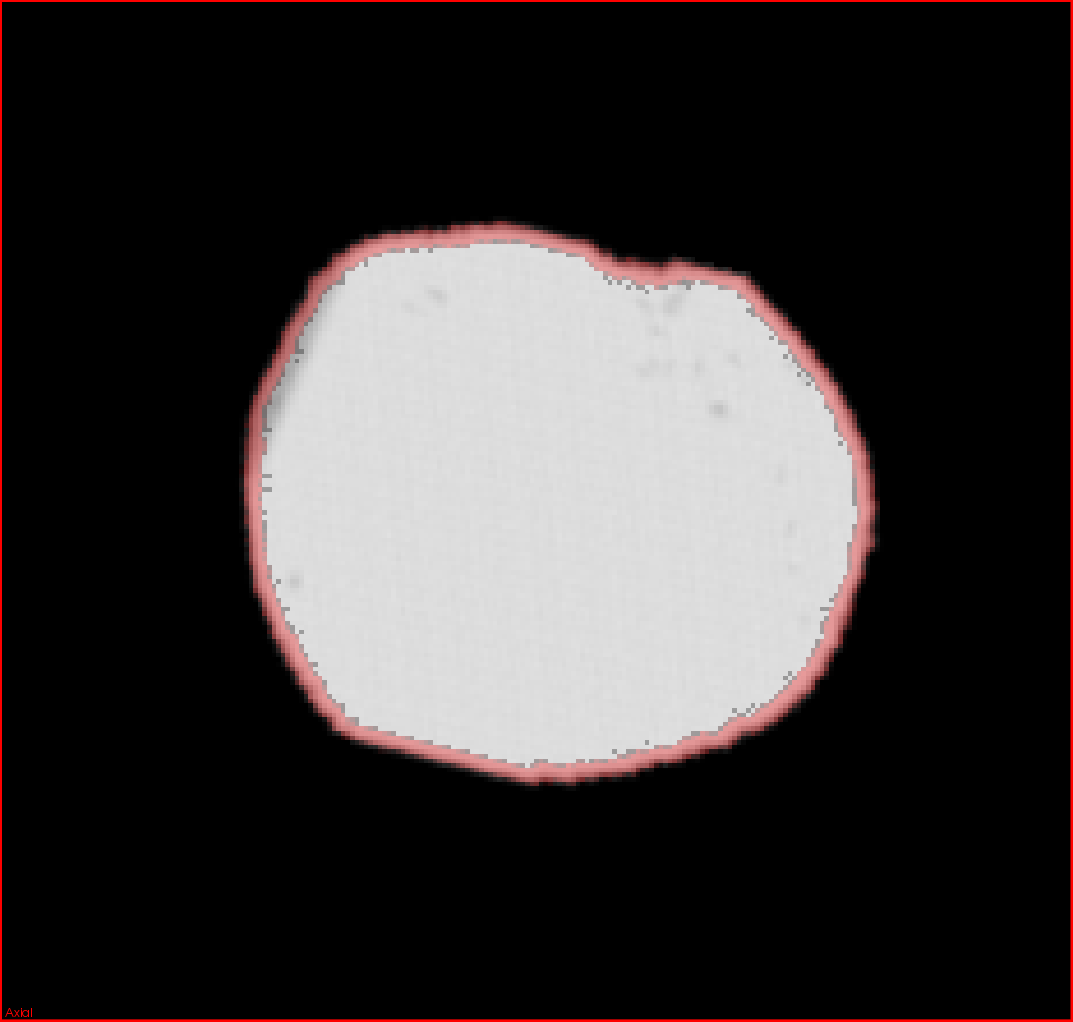
\includegraphics[width=\textwidth]{images/erosion/erosion_3.png}
    \caption{Step 3}
    \label{fig:erosion3}
  \end{subfigure}%
  ~ %add desired spacing between images, e. g. ~, \quad, \qquad, \hfill etc.
    %(or a blank line to force the subfigure onto a new line)
  \begin{subfigure}[b]{0.3\textwidth}
    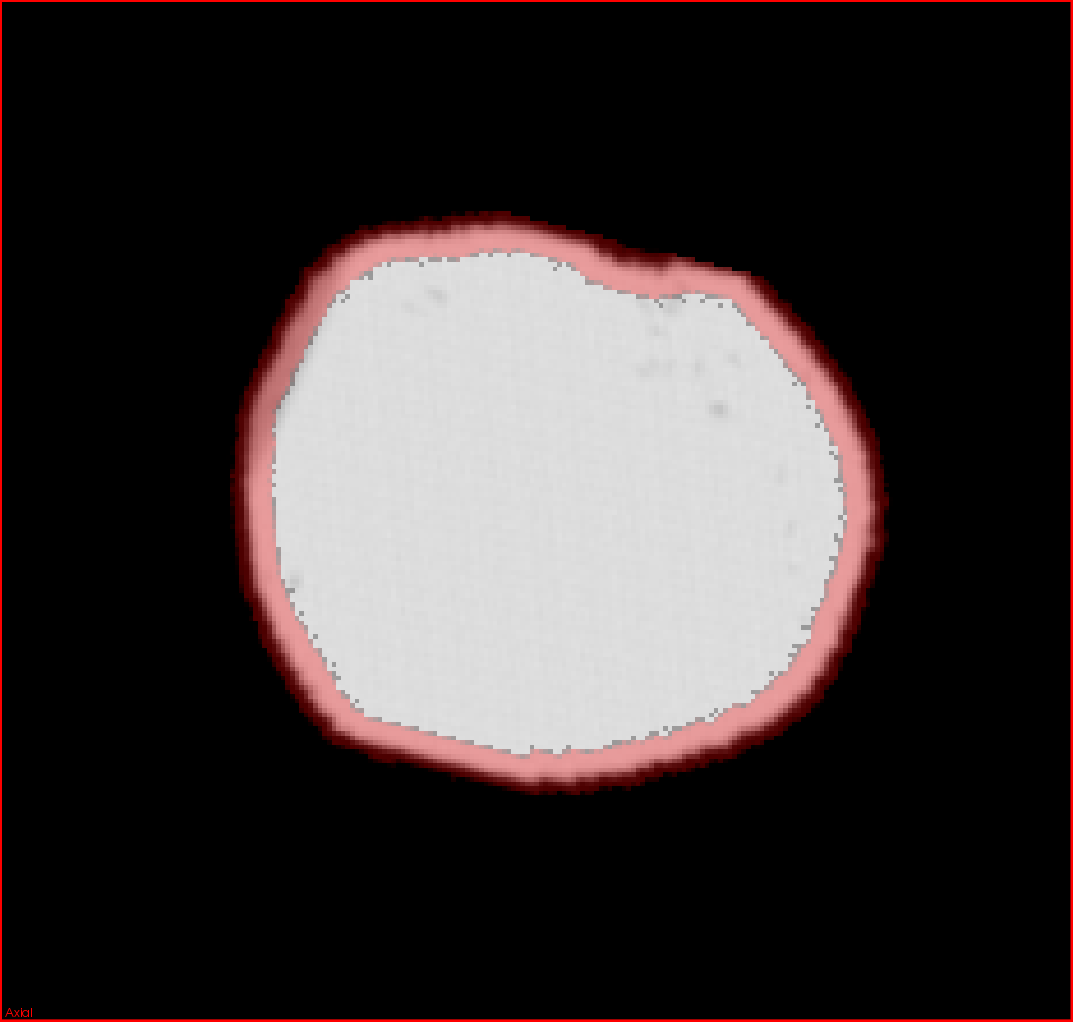
\includegraphics[width=\textwidth]{images/erosion/erosion_4.png}
    \caption{Step 4}
    \label{fig:erosion4}
  \end{subfigure}  
  ~ %add desired spacing between images, e. g. ~, \quad, \qquad, \hfill etc.
    %(or a blank line to force the subfigure onto a new line)
  \begin{subfigure}[b]{0.3\textwidth}
    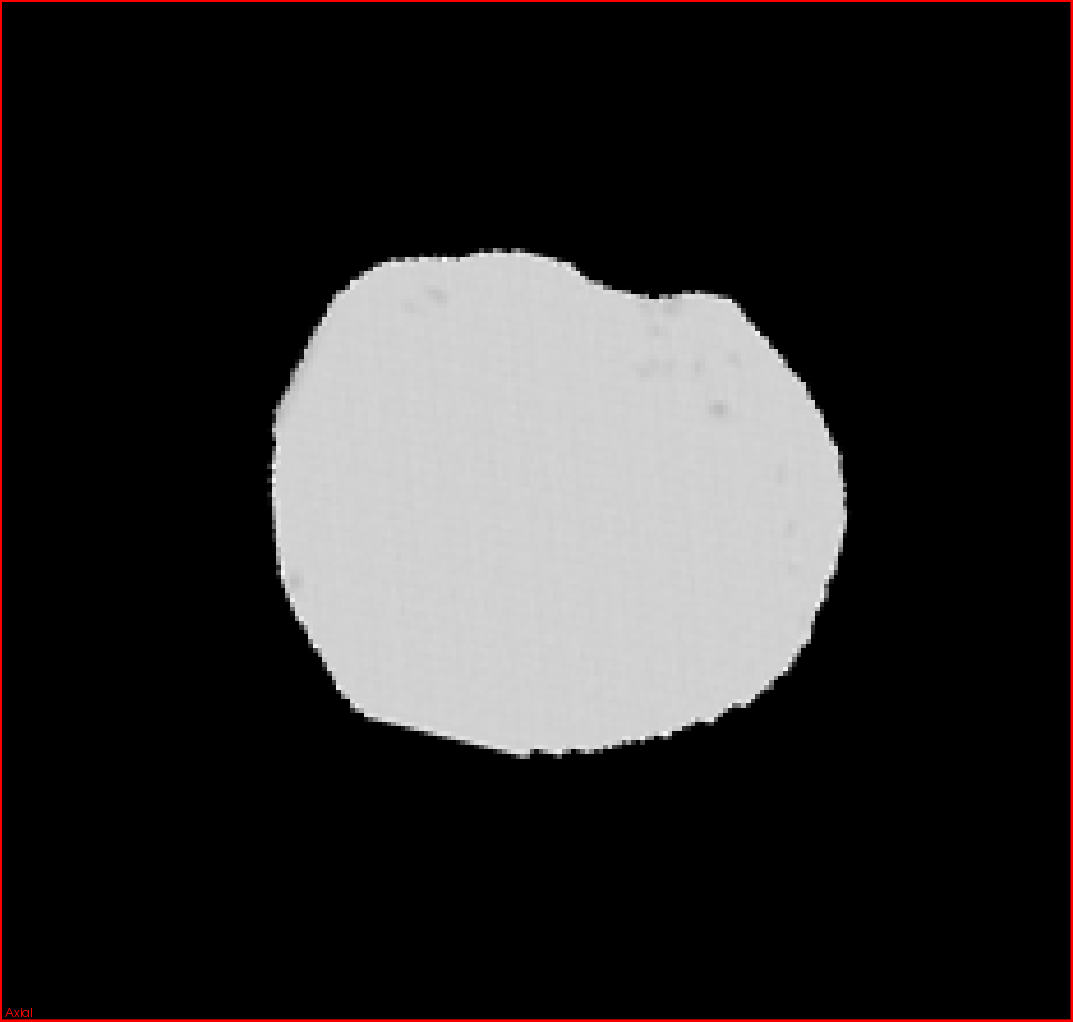
\includegraphics[width=\textwidth]{images/erosion/erosion_5.png}
    \caption{Step 5}
    \label{fig:erosion5}
  \end{subfigure}  
  \caption{Steps involved in removing the edge.}\label{fig:erosionoverview}
\end{figure}

\newpage
\section{Test Uncertainties}\label{section:testuncertainties}

To test the different visualizations during development a number of artificial uncertainty volumes were used, as well as uncertainty from a fetal brain reconstruction.

For each visualization that has been developed the results with these test uncertainties will be examined and compared.

\subsection*{Sphere of Uncertainty}
An uncertainty volume where the uncertainty is proportional to the distance from the center. The uncertainty at the center is 0 (very uncertain) which then goes to 1 (very certain) at the edges.

\subsection*{Sphere in Corner}
Similar to the sphere, but instead of being placed in the middle it is placed in one corner of the volume.

\subsection*{Cube of Uncertainty}
An uncertainty volume that is 1 (very good) everywhere except for fixed size cube of uncertainty 0 (very bad) in the center.

\subsection*{Random Uncertainty}
The uncertainty at every point is a random uniformly distributed value.

\subsection*{Reconstruction Uncertainty}
Uncertainty generated from an example super resolution reconstruction of a fetal brain.\\

\begin{figure}[h]
  \centering
  \begin{subfigure}[b]{0.18\textwidth}
    \fcolorbox{gray}{white}{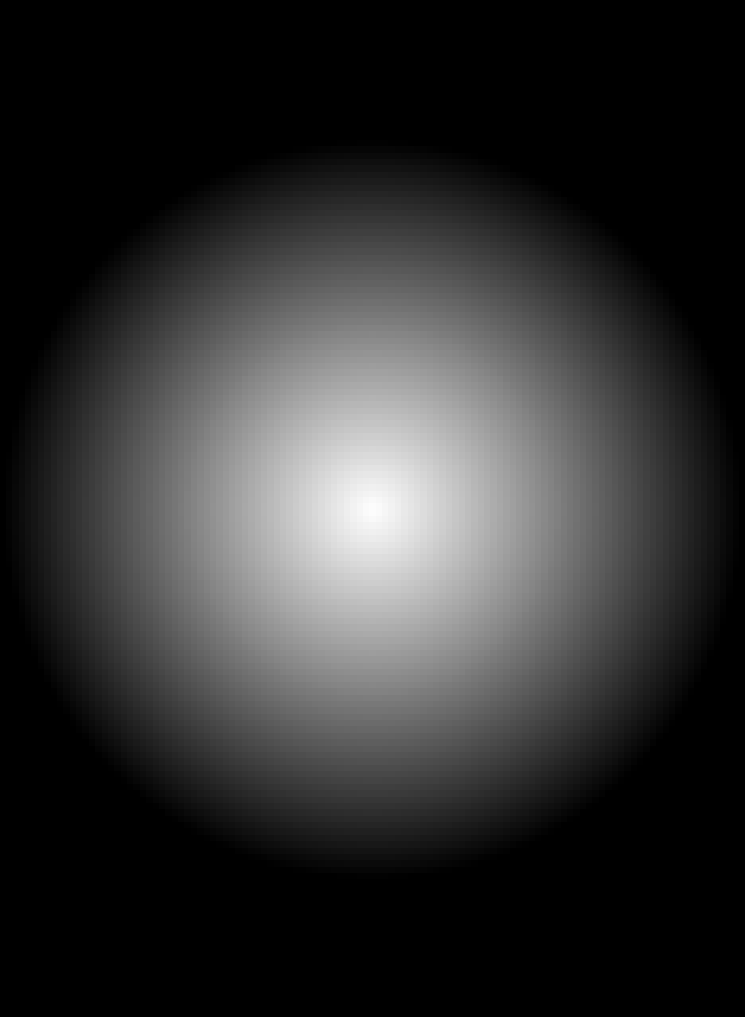
\includegraphics[width=\textwidth]{images/test/test_sphere.png}}
    \caption{Sphere}
    \label{fig:erosion0}
  \end{subfigure}%
  ~~%add desired spacing between images, e. g. ~, \quad, \qquad, \hfill etc.
    %(or a blank line to force the subfigure onto a new line)
  \begin{subfigure}[b]{0.18\textwidth}
    \fcolorbox{gray}{white}{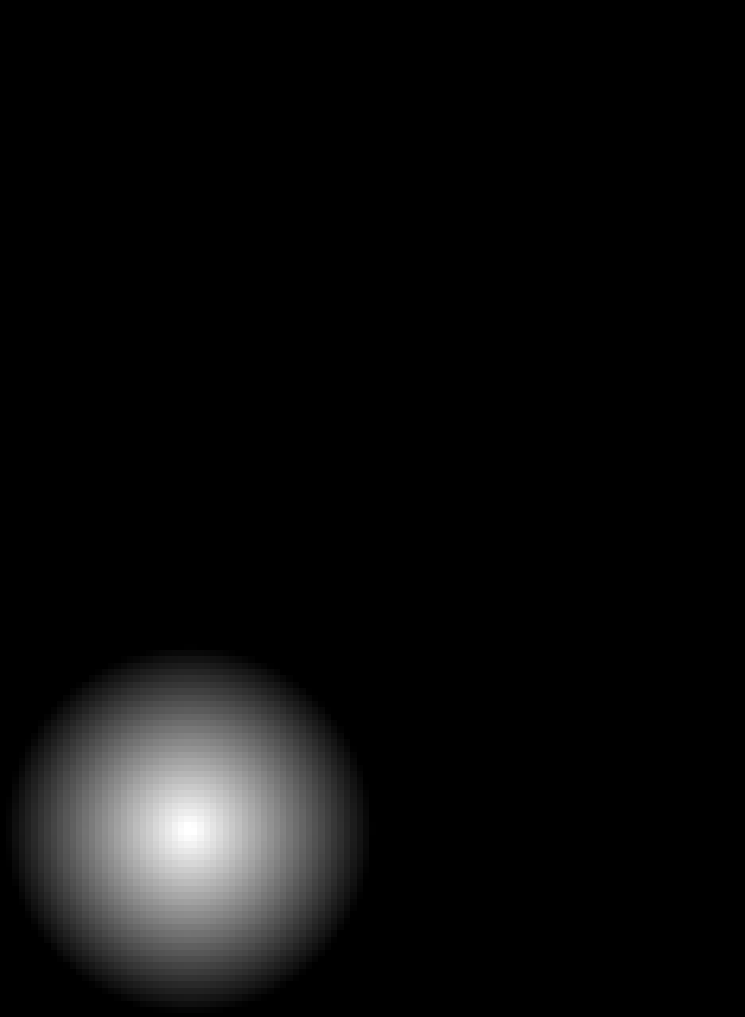
\includegraphics[width=\textwidth]{images/test/test_quadsphere.png}}
    \caption{Corner}
    \label{fig:erosion1}
  \end{subfigure}%
  ~~%add desired spacing between images, e. g. ~, \quad, \qquad, \hfill etc.
    %(or a blank line to force the subfigure onto a new line)
  \begin{subfigure}[b]{0.18\textwidth}
    \fcolorbox{gray}{white}{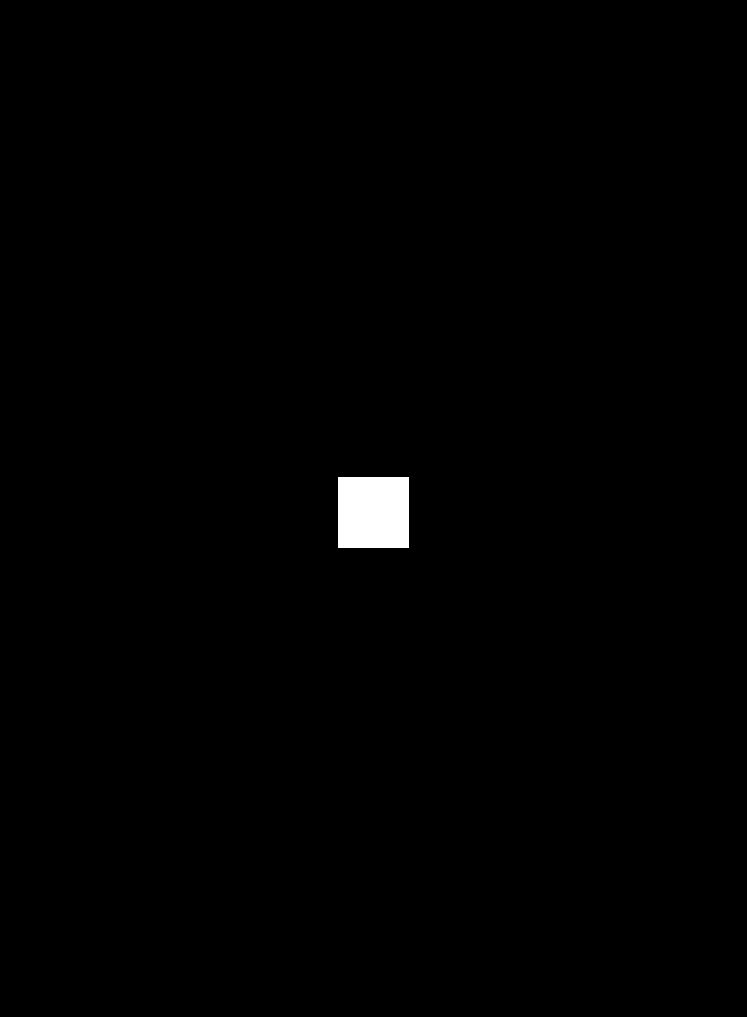
\includegraphics[width=\textwidth]{images/test/test_cube.png}}
    \caption{Cube}
    \label{fig:erosion2}
  \end{subfigure}%
  ~~%add desired spacing between images, e. g. ~, \quad, \qquad, \hfill etc.
    %(or a blank line to force the subfigure onto a new line)
  \begin{subfigure}[b]{0.18\textwidth}
    \fcolorbox{gray}{white}{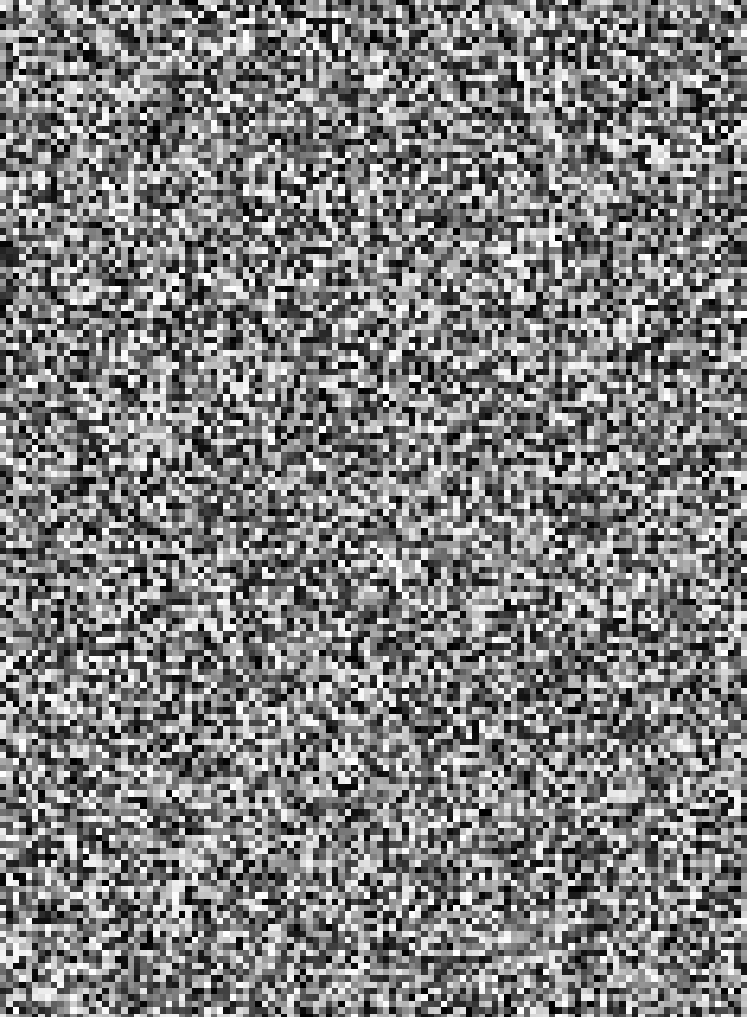
\includegraphics[width=\textwidth]{images/test/test_random.png}}
    \caption{Random}
    \label{fig:erosion3}
  \end{subfigure}%
  ~~%add desired spacing between images, e. g. ~, \quad, \qquad, \hfill etc.
    %(or a blank line to force the subfigure onto a new line)
  \begin{subfigure}[b]{0.18\textwidth}
    \fcolorbox{gray}{white}{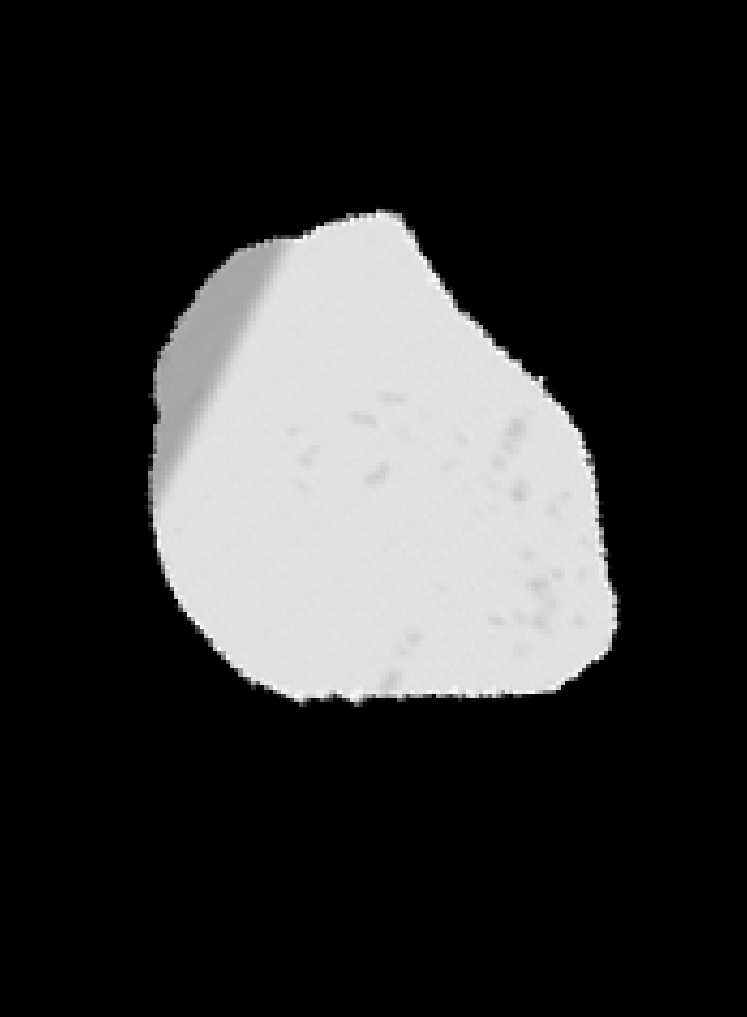
\includegraphics[width=\textwidth]{images/test/test_scan.png}}
    \caption{Fetal Brain}
    \label{fig:erosion3}
  \end{subfigure}
  \caption{Steps involved in removing the edge.}\label{fig:erosionoverview}
\end{figure}

% Idea -> Implementation -> Results
\newpage
\section{Thresholding}\label{section:thresholding}

The idea behind thresholding is to isolate areas in the reconstructed image within a particular range of uncertainty. This allows the viewer to highlight regions in a specified range (e.g. 0.2 to 0.5) and also lets them isolate the worst values in the volume (e.g. the worst 1$\%$).

\subsection*{Implementation}
The implementation uses a filter provided by ITK to go create a binary mask which is set to 1 where the uncertainty is in the range and 0 where it is not. This mask is then overlayed on the reconstructed scan in 2D and made transparent so both the uncertain area and underlying scan can be seen simultaneously. See figure \ref{fig:thresholding2d}.

\begin{figure}[H]
  \centering
  \begin{subfigure}[b]{0.3\textwidth}
    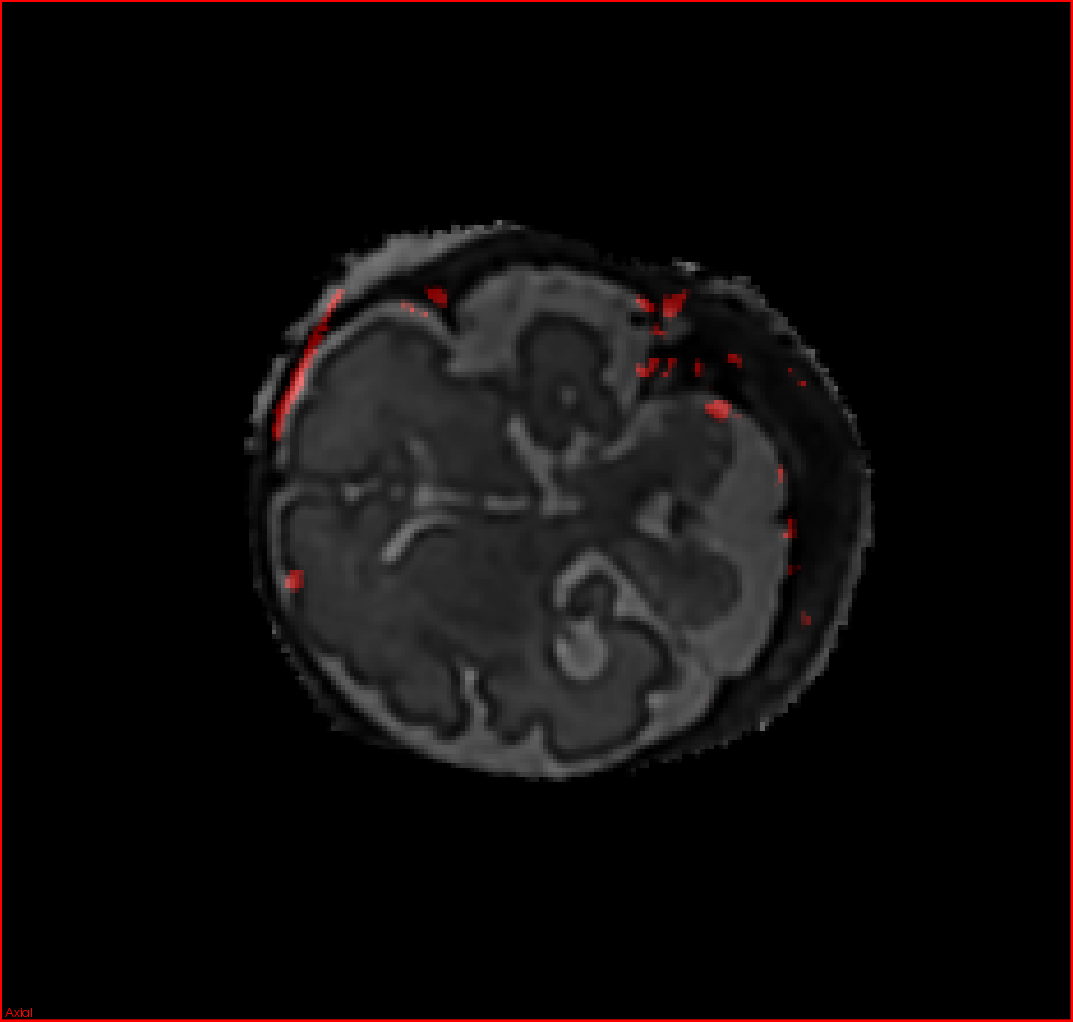
\includegraphics[width=\textwidth]{images/thresholding/thresholding_2d_axial.png}
    \caption{Axial}
    \label{fig:thresholding2daxial}
  \end{subfigure}%
  ~ %add desired spacing between images, e. g. ~, \quad, \qquad, \hfill etc.
    %(or a blank line to force the subfigure onto a new line)
  \begin{subfigure}[b]{0.3\textwidth}
    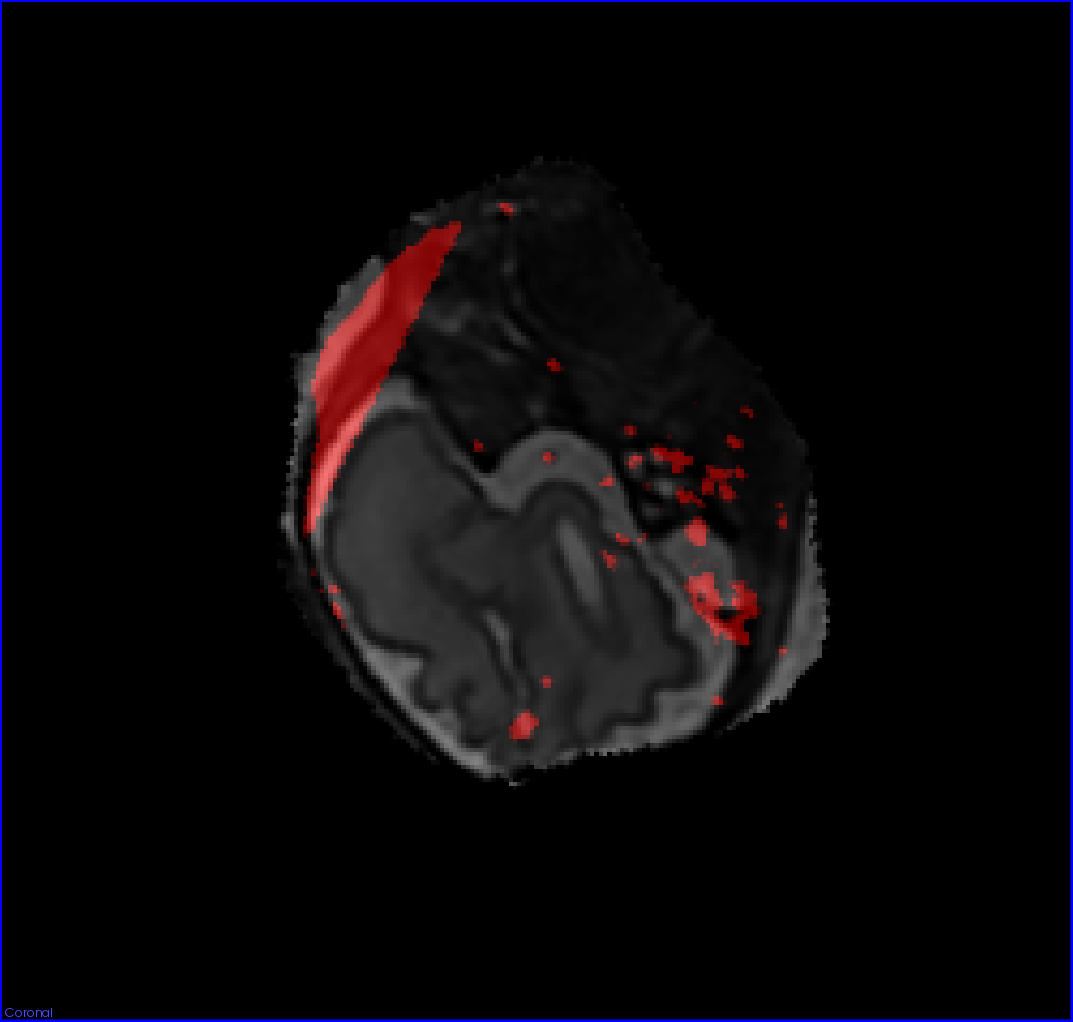
\includegraphics[width=\textwidth]{images/thresholding/thresholding_2d_coronal.png}
    \caption{Coronal}
    \label{fig:thresholding2dcoronal}
  \end{subfigure}%
  ~ %add desired spacing between images, e. g. ~, \quad, \qquad, \hfill etc.
    %(or a blank line to force the subfigure onto a new line)
  \begin{subfigure}[b]{0.3\textwidth}
    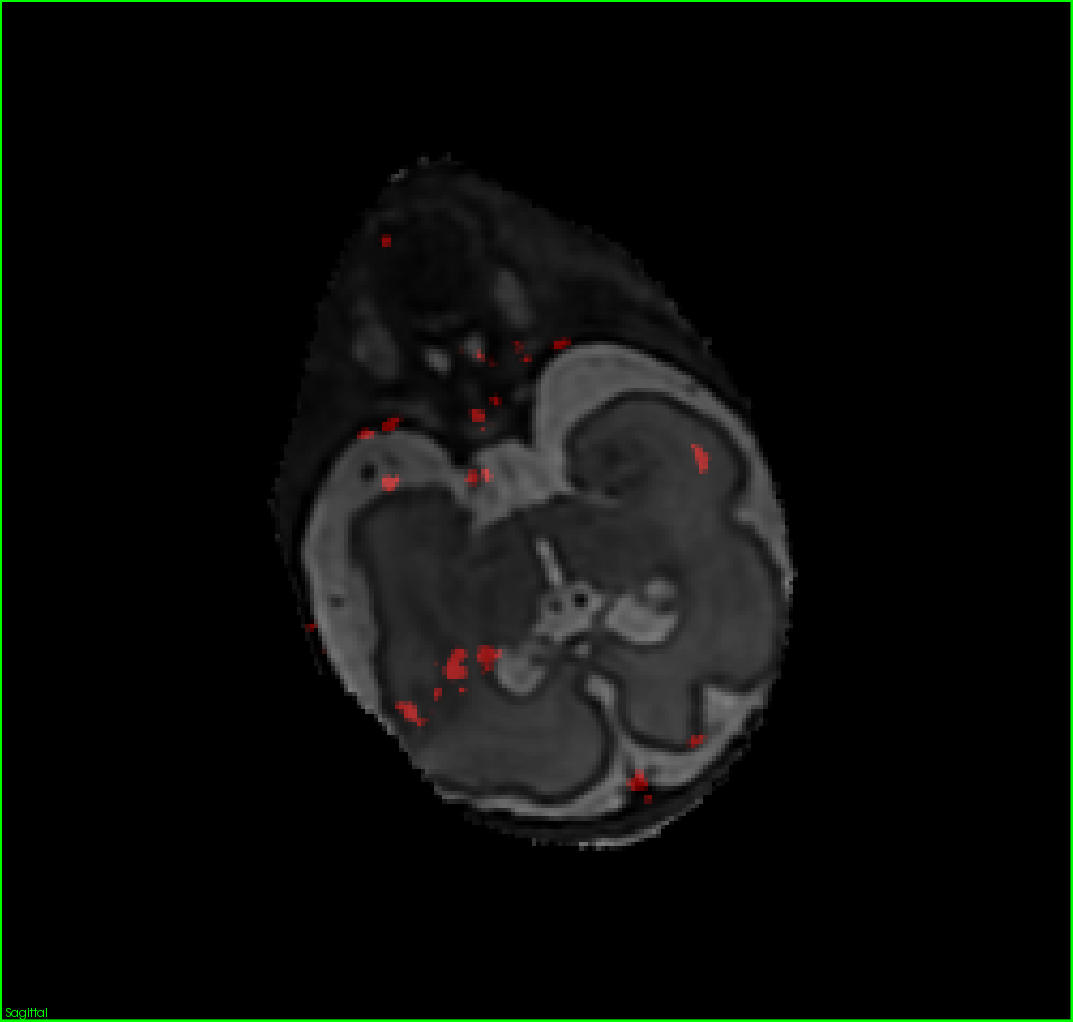
\includegraphics[width=\textwidth]{images/thresholding/thresholding_2d_sagittal.png}
    \caption{Sagittal}
    \label{fig:thresholding2dsagittal}  
  \end{subfigure}
  \caption{Thresholding in 2D}\label{fig:thresholding2d}
\end{figure}

To view the uncertainty in 3D, two variations have been implemented, both using volume rendering (see section \ref{background:volumerendering}). Variation 1 applies volume rendering directly to the uncertainty and variation 2 applies volume rendering to the binary mask.

The transfer functions used in each variation can be seen in figure \ref{fig:thresholdingoverview}. The first works by making values within the thresholded range opaque and those outside it transparent. The second works in a similar way; 0 in the mask is out of the range and 1 in the mask is in the range. In the second transfer function there is a slow fade out, rather than a sharp change, to give individual points of uncertainty some presence.

\begin{figure}[H]
  \centering
  \begin{subfigure}[b]{0.5\textwidth}
    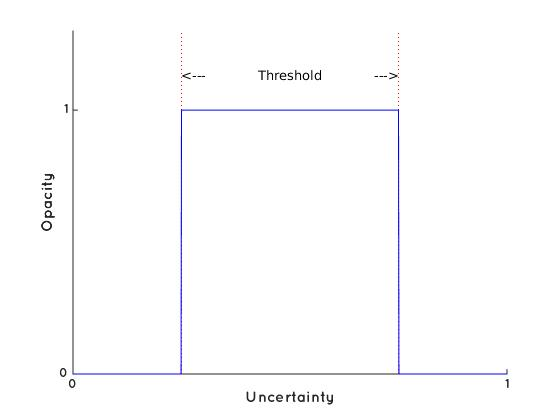
\includegraphics[width=\textwidth]{images/thresholding/thresholdvariation1.jpg}
    \caption{Variation 1}
    \label{fig:thresholdingvariation1}
  \end{subfigure}%
  ~ %add desired spacing between images, e. g. ~, \quad, \qquad, \hfill etc.
    %(or a blank line to force the subfigure onto a new line)
  \begin{subfigure}[b]{0.5\textwidth}
    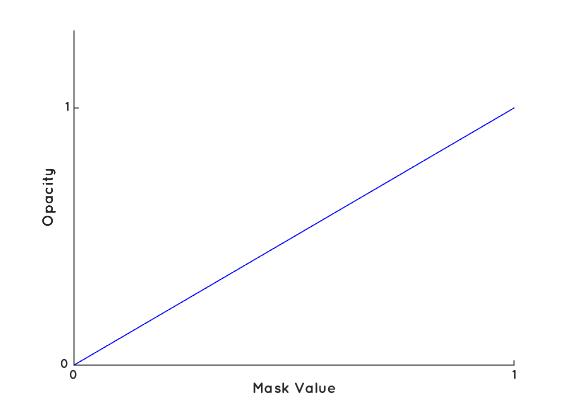
\includegraphics[width=\textwidth]{images/thresholding/thresholdvariation2.jpg}
    \caption{Variation 2}
    \label{fig:thresholdingvariation2}
  \end{subfigure}
  \caption{Opacity Transfer Functions. Opacity of 0 is transparent, 1 is opaque.}\label{fig:thresholdingoverview}
\end{figure}

An issue found with variation 1 was that the renderer still draws the edge of the uncertainty, even though it had previously been removed by erosion. This is due to the renderer using linear interpolation to take samples along each ray fired into the volume. Figure \ref{fig:thresholdingvariation1problem} illustrates the problem - the background has uncertainty 0.0, and the object has uncertainty $~$0.6. Points interpolated between the two will lie in the range 0.0-0.6 and so we find values of uncertainty that don't actually exist in the object.

\begin{figure}[h]
  \centering
  \begin{subfigure}[b]{0.5\textwidth}
    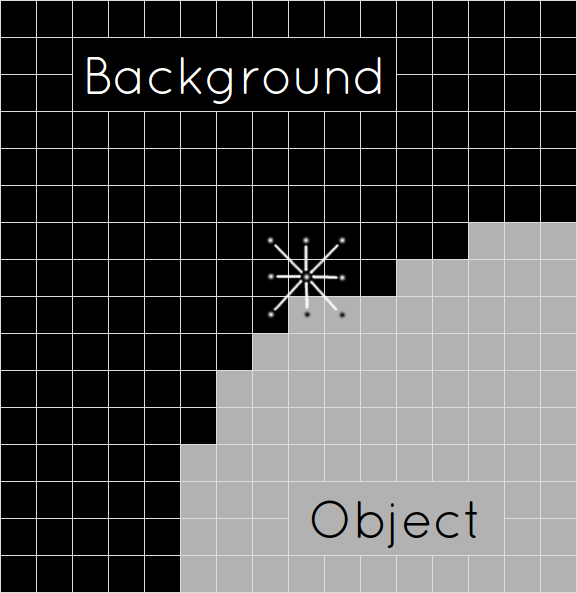
\includegraphics[width=\textwidth]{images/thresholding/thresholdvariation1example.png}
    \caption{Simplified View}
    \label{fig:thresholdingvariation1example}
  \end{subfigure}%
  ~ %add desired spacing between images, e. g. ~, \quad, \qquad, \hfill etc.
    %(or a blank line to force the subfigure onto a new line)
  \begin{subfigure}[b]{0.5\textwidth}
    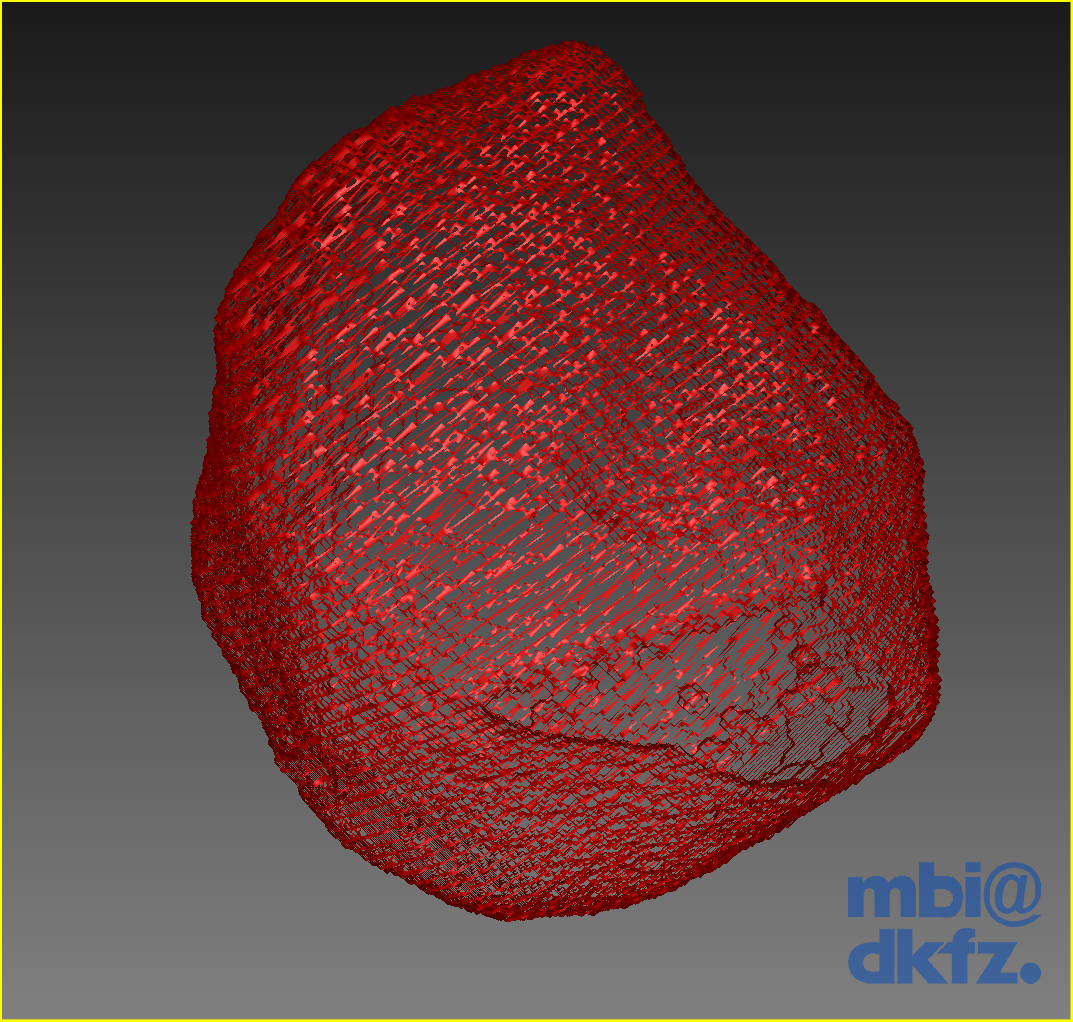
\includegraphics[width=\textwidth]{images/thresholding/thresholdvariation1problem.png}
    \caption{Edge Artefacts}
    \label{fig:thresholdingvariation1artefacts}
  \end{subfigure}
  \caption{Opacity Transfer Functions. Opacity of 0 is transparent, 1 is opaque.}\label{fig:thresholdingvariation1problem}
\end{figure}

A solution to this problem is to use a gradient transfer function which allows the change in uncertainty to influence the transparency. Rapid changes in uncertainty can therefore be treated as noise and ignored. The cutoff can be adjusted to remove the entire edge but there is a tradeoff as some genuine regions of uncertainty can also be filteredout. Figure \ref{fig:thresholdingvariationfix} shows the transfer function and the effect of tweaking the threshold.

\begin{figure}[H]
  \centering
  \begin{subfigure}[b]{0.5\textwidth}
    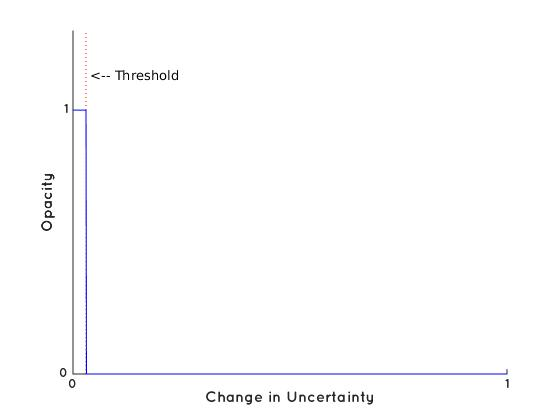
\includegraphics[width=\textwidth]{images/thresholding/thresholdvariation1fix.jpg}
    \caption{Gradient Transfer Function}
    \label{fig:thresholdingvariation1example}
  \end{subfigure}%
  ~ %add desired spacing between images, e. g. ~, \quad, \qquad, \hfill etc.
    %(or a blank line to force the subfigure onto a new line)
  \begin{subfigure}[b]{0.5\textwidth}
    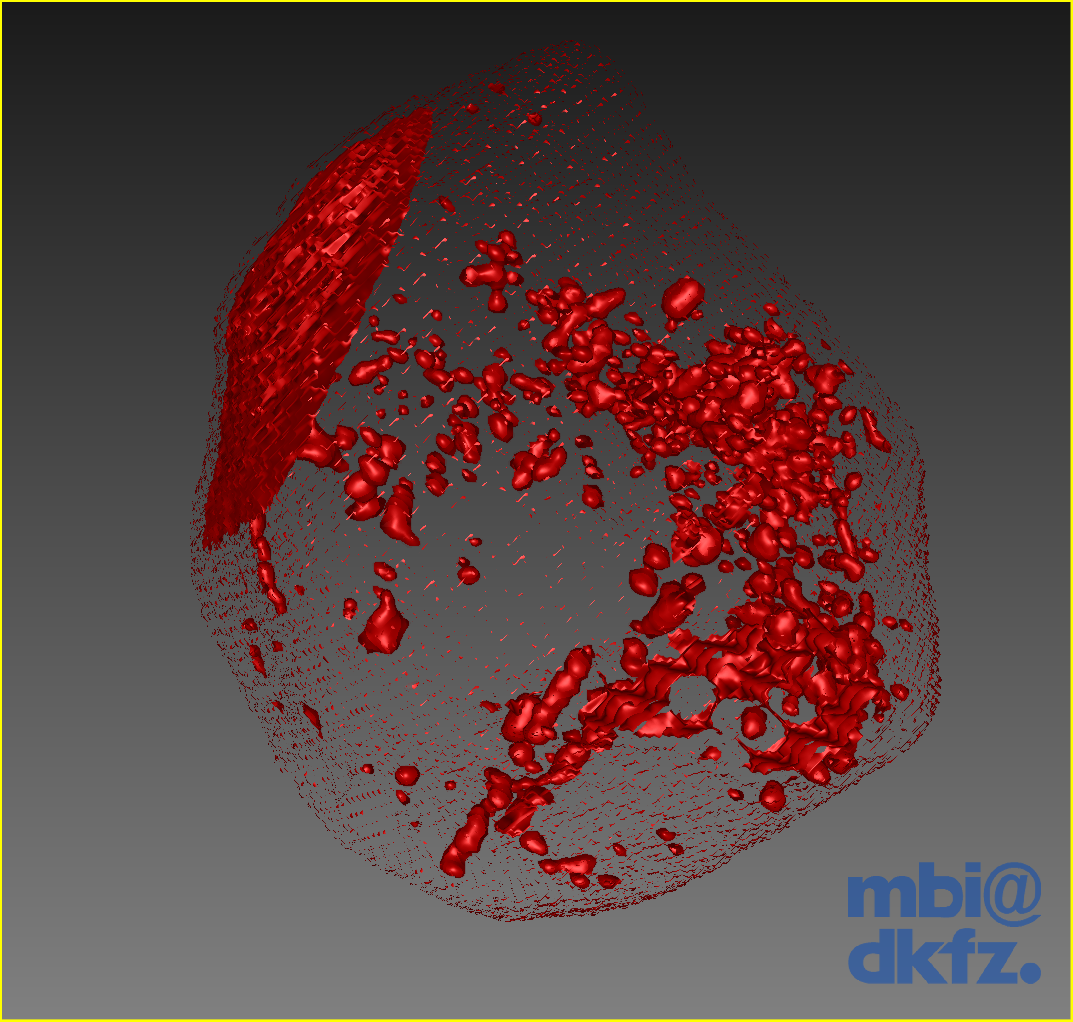
\includegraphics[width=\textwidth]{images/thresholding/thresholdvariation1threshold1.png}
    \caption{Threshold 0.05}
    \label{fig:thresholdingvariation1threshold1}
  \end{subfigure}
  ~%add desired spacing between images, e. g. ~, \quad, \qquad, \hfill etc.
    %(or a blank line to force the subfigure onto a new line)
  \begin{subfigure}[b]{0.5\textwidth}
    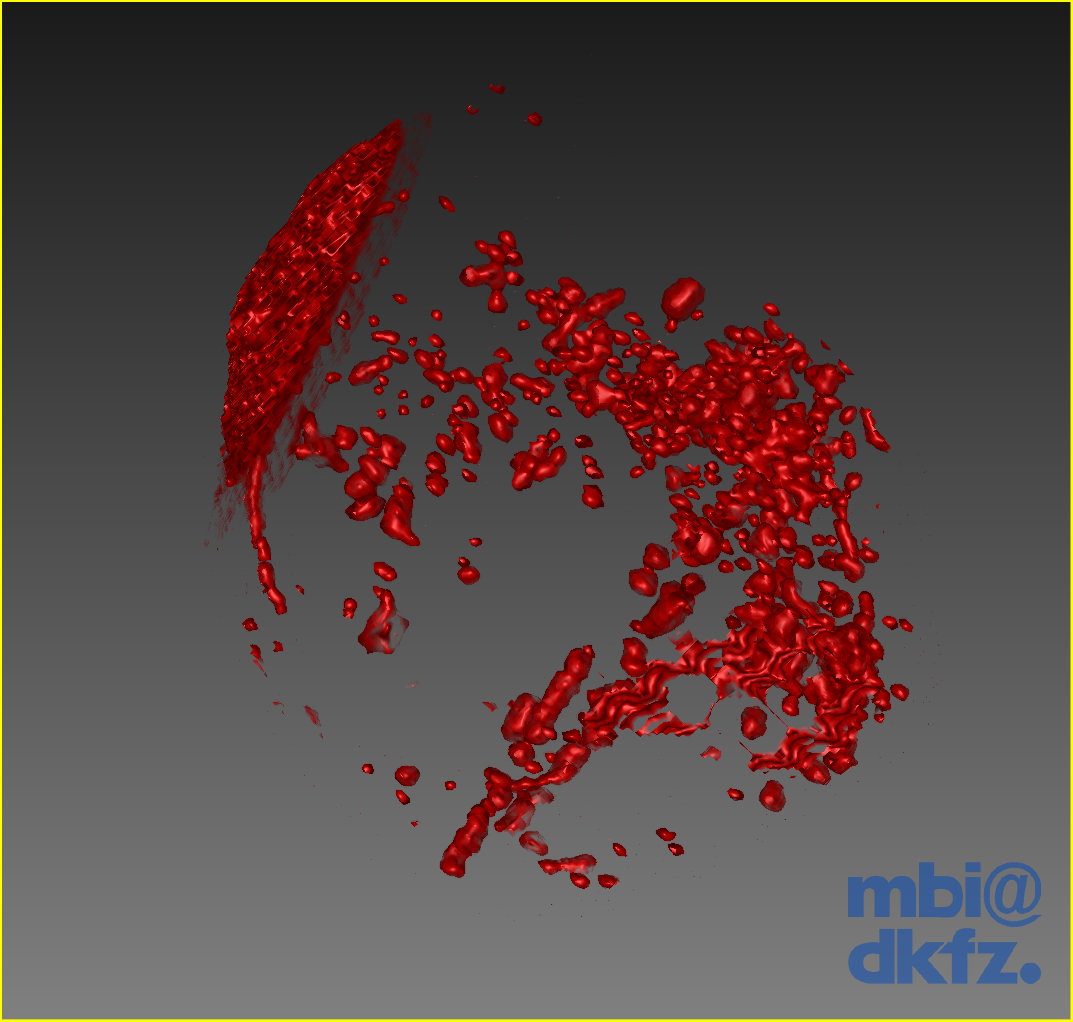
\includegraphics[width=\textwidth]{images/thresholding/thresholdvariation1threshold2.png}
    \caption{Threshold 0.02}
    \label{fig:thresholdingvariation1threshold2}  
  \end{subfigure}%
  ~ %add desired spacing between images, e. g. ~, \quad, \qquad, \hfill etc.
    %(or a blank line to force the subfigure onto a new line)
  \begin{subfigure}[b]{0.5\textwidth}
    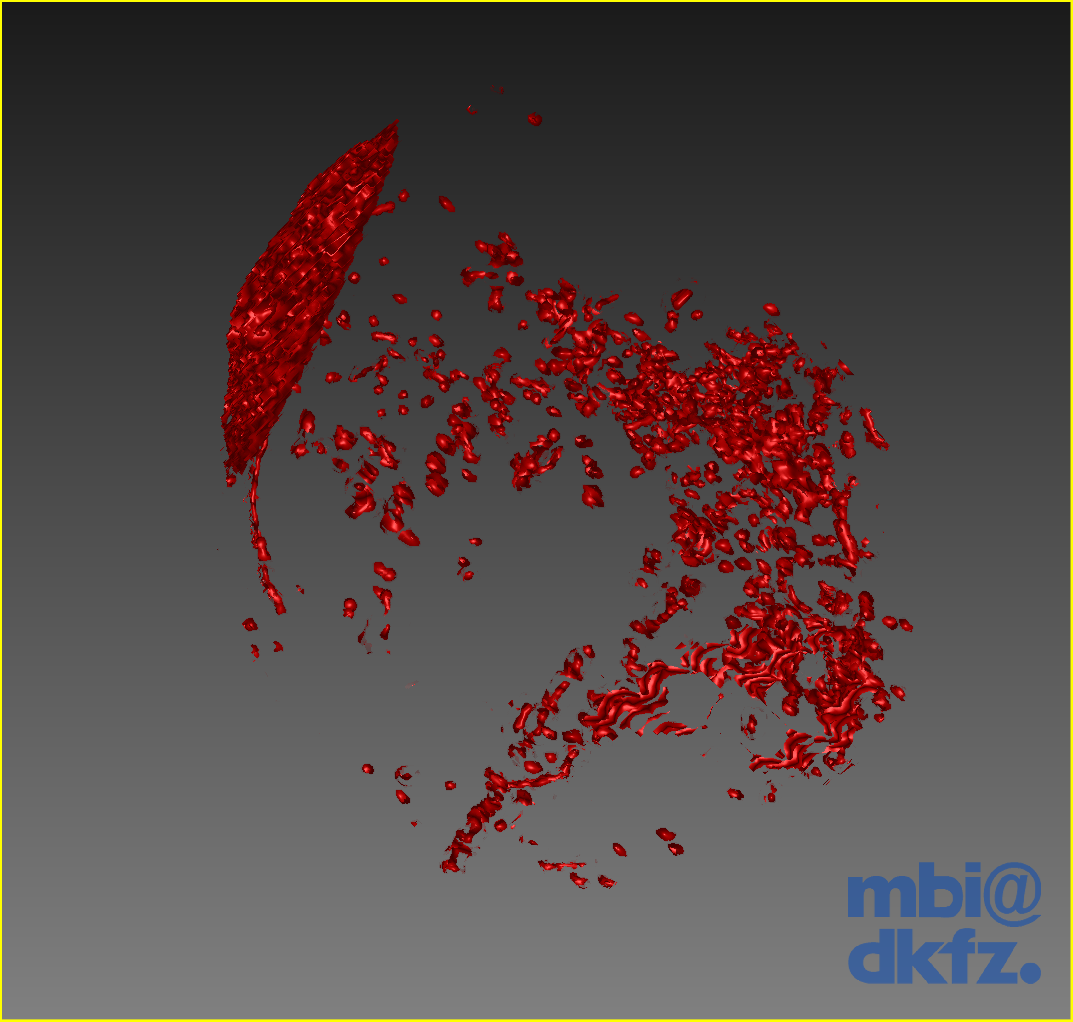
\includegraphics[width=\textwidth]{images/thresholding/thresholdvariation1threshold3.png}
    \caption{Threshold 0.01}
    \label{fig:thresholdingvariation1threshold3}  
  \end{subfigure}  
  \caption{Reducing the threshold removes the edge but removes some uncertainty.}\label{fig:thresholdingvariationfix}
\end{figure}

Although tweaking the threshold can remove edge artefact variation 2 was found not to exhibit these problems and so this implementation was used in the evaluation of the prototype.

\newpage
\subsection*{Results}
Here are the results that are achieved with the test uncertainties (see section \ref{section:testuncertainties}).

\begin{figure}[H]
  \centering
  \begin{subfigure}[b]{0.32\textwidth}
    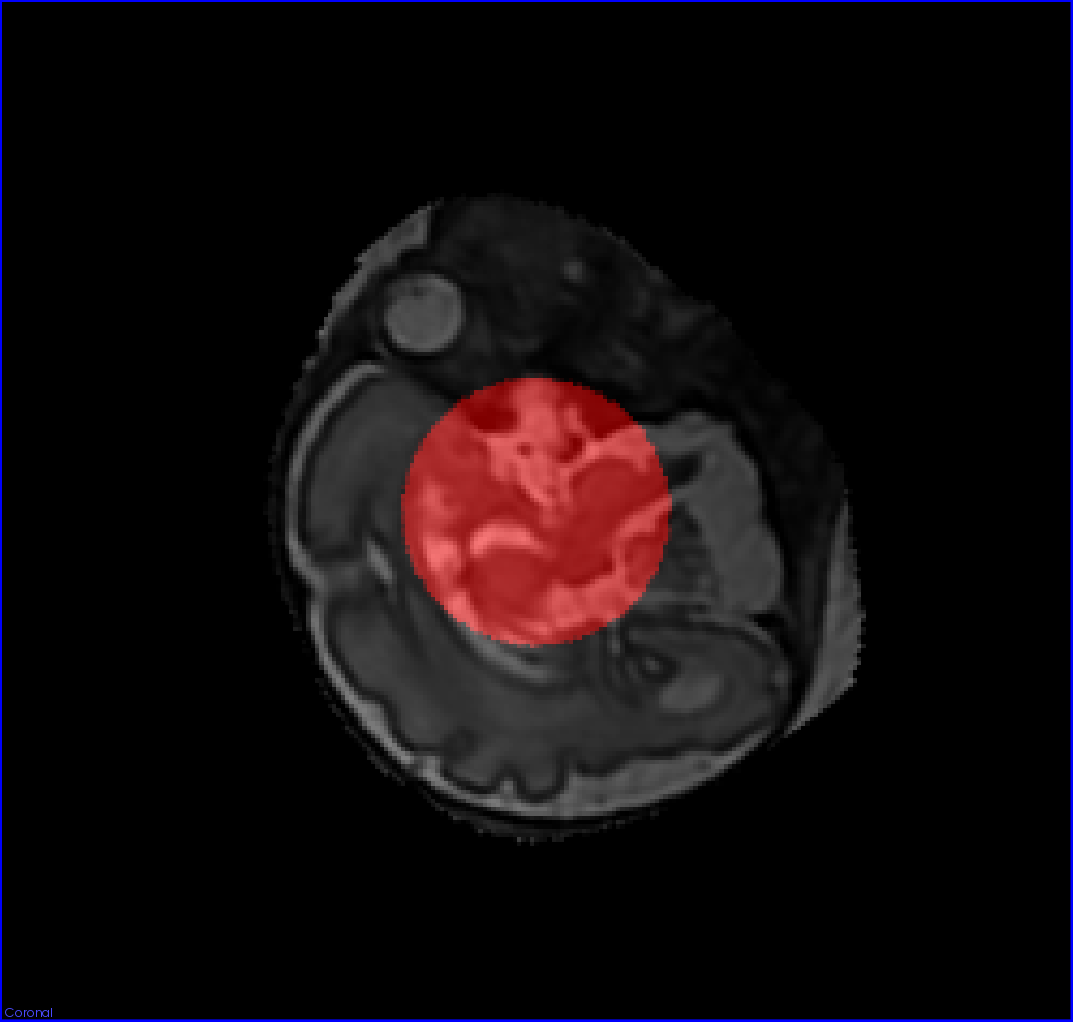
\includegraphics[width=\textwidth]{images/thresholding/results/sphere_2d.png}
    \caption{Sphere in 2D}
    \label{fig:thresholdingresultssphere2d}
  \end{subfigure}%
  ~ %add desired spacing between images, e. g. ~, \quad, \qquad, \hfill etc.
    %(or a blank line to force the subfigure onto a new line)
  \begin{subfigure}[b]{0.32\textwidth}
    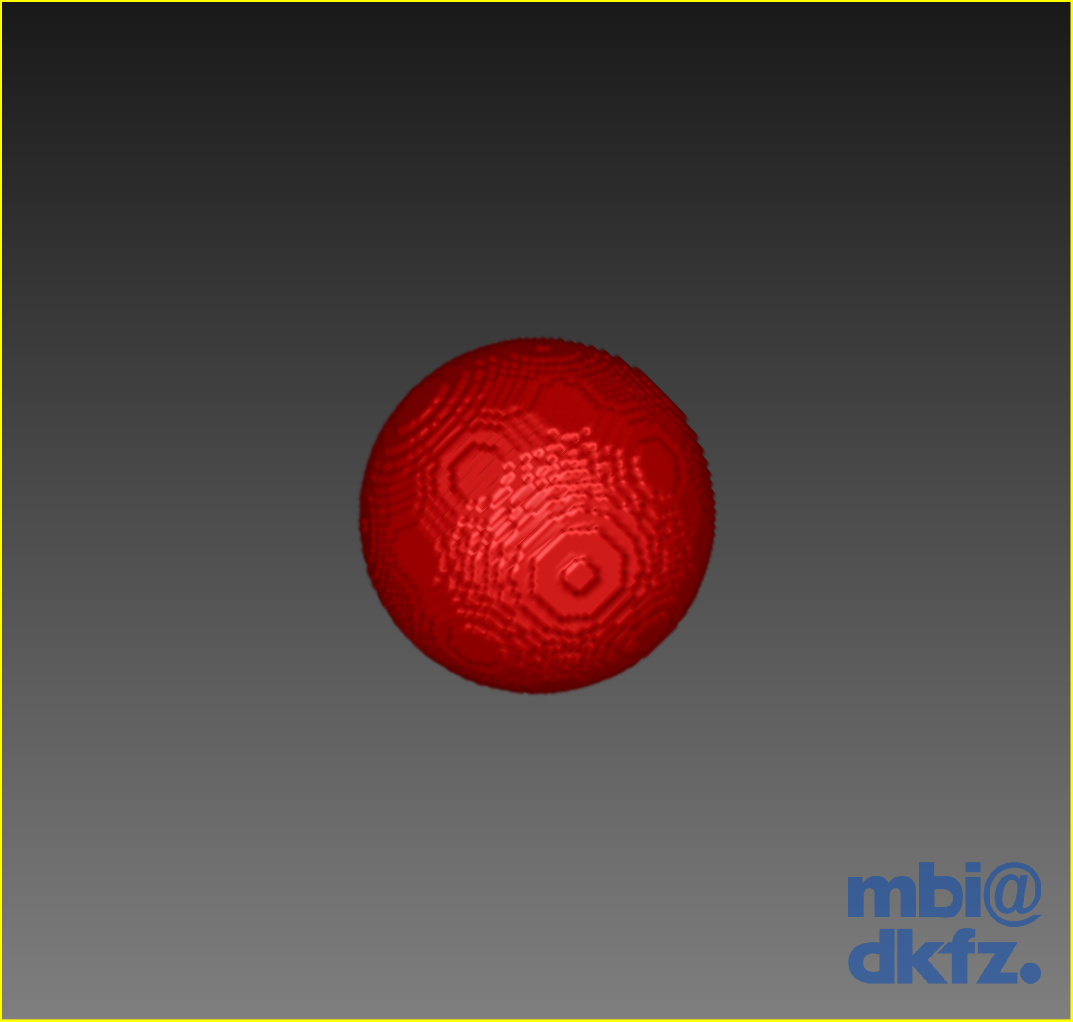
\includegraphics[width=\textwidth]{images/thresholding/results/sphere_3d.png}
    \caption{Sphere in 3D}
    \label{fig:thresholdingresultssphere3d}
  \end{subfigure}
  ~ %add desired spacing between images, e. g. ~, \quad, \qquad, \hfill etc.
    %(or a blank line to force the subfigure onto a new line)
  \begin{subfigure}[b]{0.32\textwidth}
    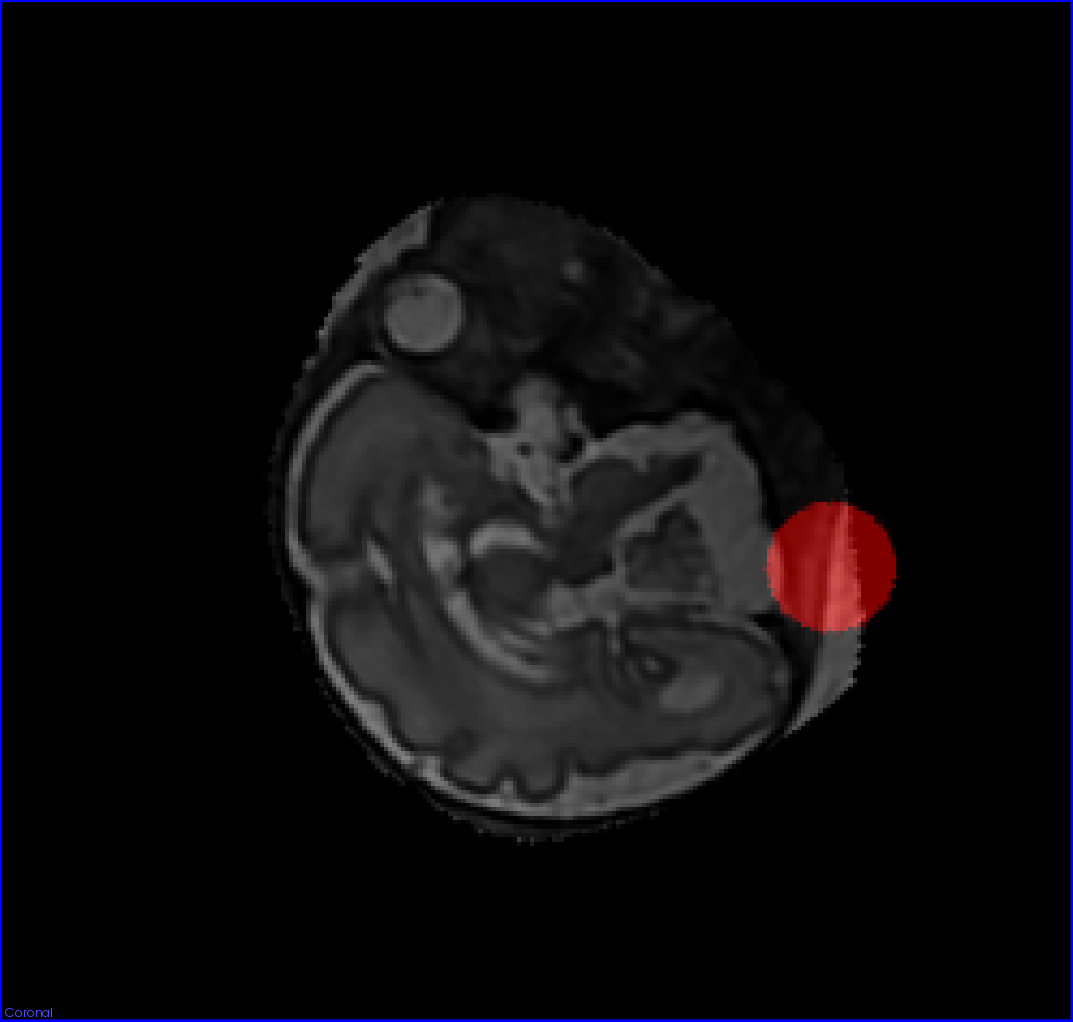
\includegraphics[width=\textwidth]{images/thresholding/results/sphere_corner_2d.png}
    \caption{Sphere in Corner in 2D}
    \label{fig:thresholdingresultsspherecorner2d}
  \end{subfigure}%
  ~ %add desired spacing between images, e. g. ~, \quad, \qquad, \hfill etc.
    %(or a blank line to force the subfigure onto a new line)
  \begin{subfigure}[b]{0.32\textwidth}
    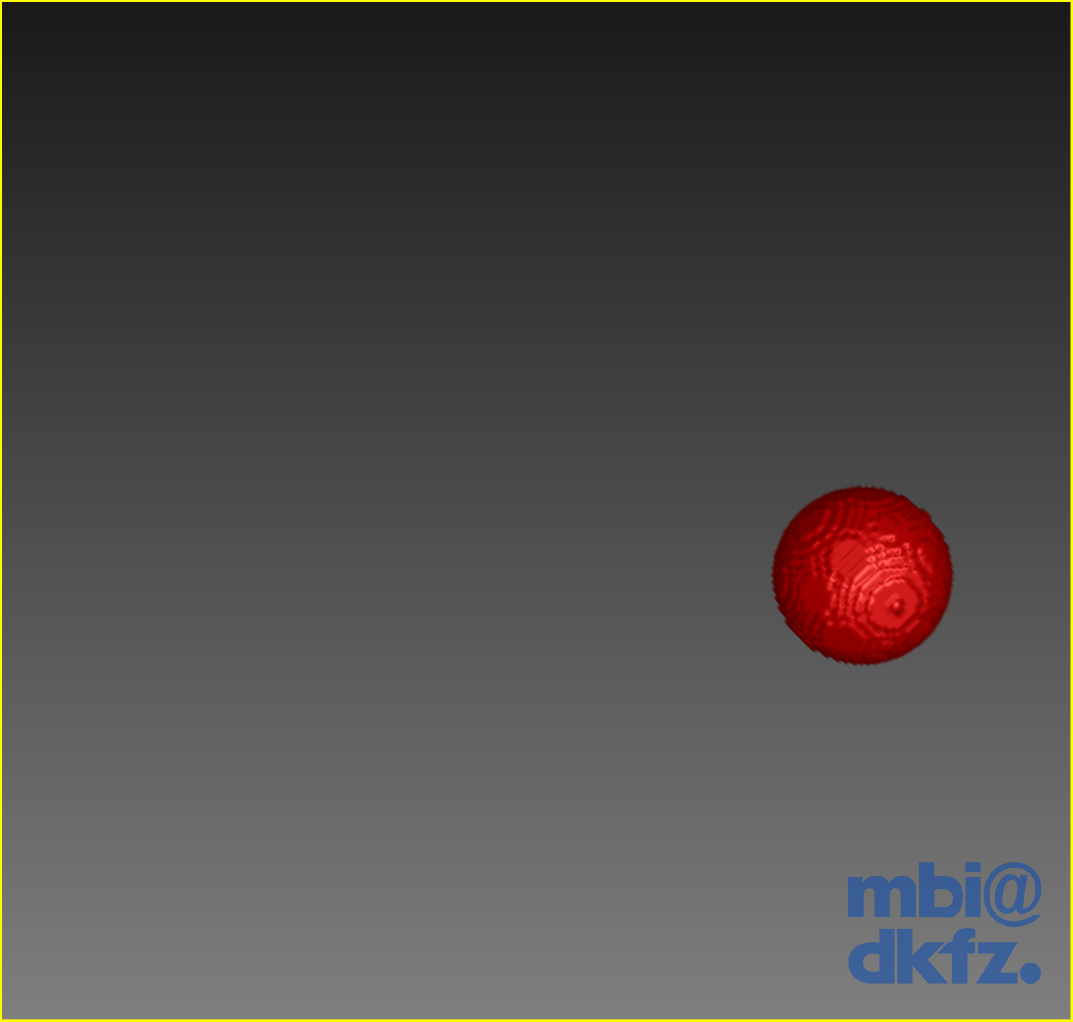
\includegraphics[width=\textwidth]{images/thresholding/results/sphere_corner_3d.png}
    \caption{Sphere in Corner in 3D}
    \label{fig:thresholdingresultsspherecorner3d}
  \end{subfigure}
  ~ %add desired spacing between images, e. g. ~, \quad, \qquad, \hfill etc.
    %(or a blank line to force the subfigure onto a new line)
  \begin{subfigure}[b]{0.32\textwidth}
    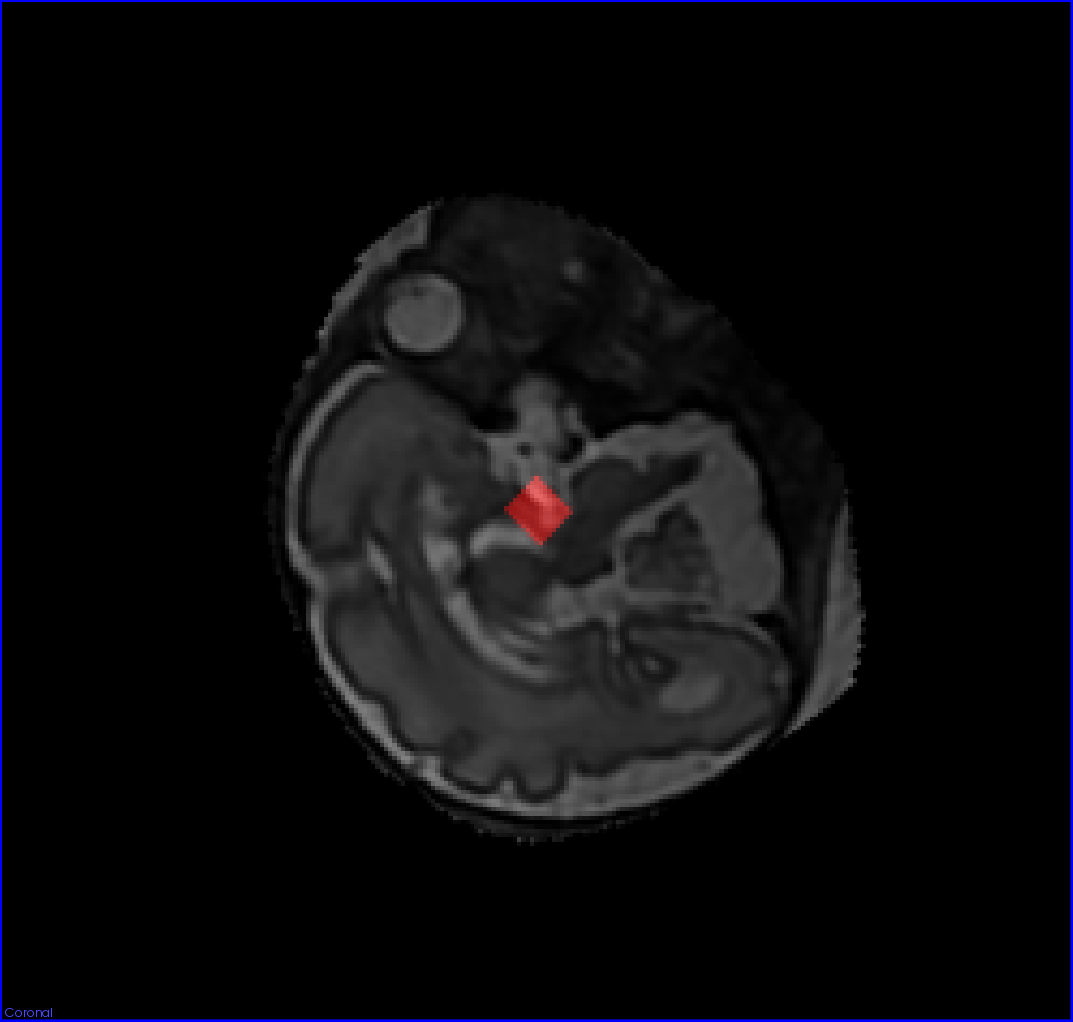
\includegraphics[width=\textwidth]{images/thresholding/results/cube_2d.png}
    \caption{Cube in 2D}
    \label{fig:thresholdingresultscube2d}
  \end{subfigure}%
  ~ %add desired spacing between images, e. g. ~, \quad, \qquad, \hfill etc.
    %(or a blank line to force the subfigure onto a new line)
  \begin{subfigure}[b]{0.32\textwidth}
    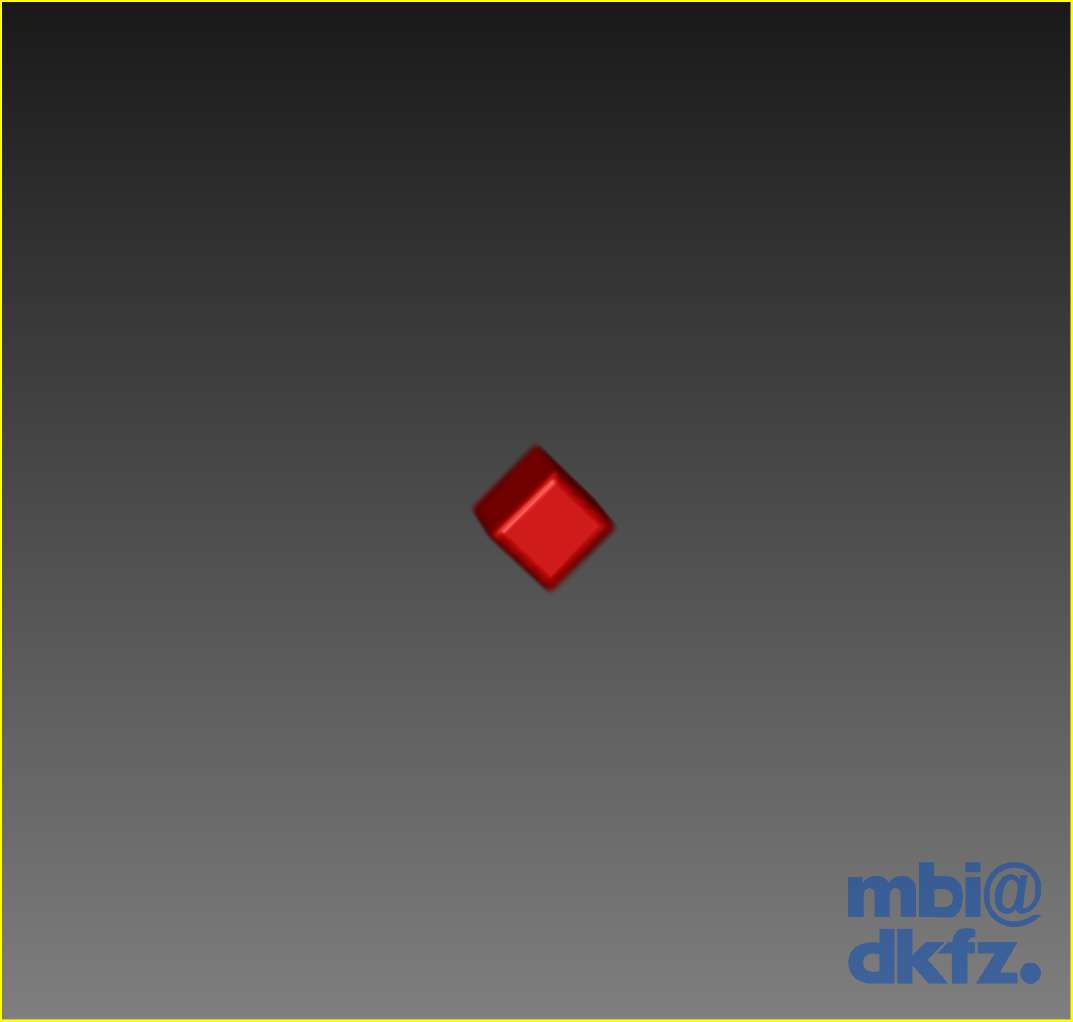
\includegraphics[width=\textwidth]{images/thresholding/results/cube_3d.png}
    \caption{Cube in 3D}
    \label{fig:thresholdingresultscube3d}
  \end{subfigure}
  ~ %add desired spacing between images, e. g. ~, \quad, \qquad, \hfill etc.
    %(or a blank line to force the subfigure onto a new line)
  \begin{subfigure}[b]{0.32\textwidth}
    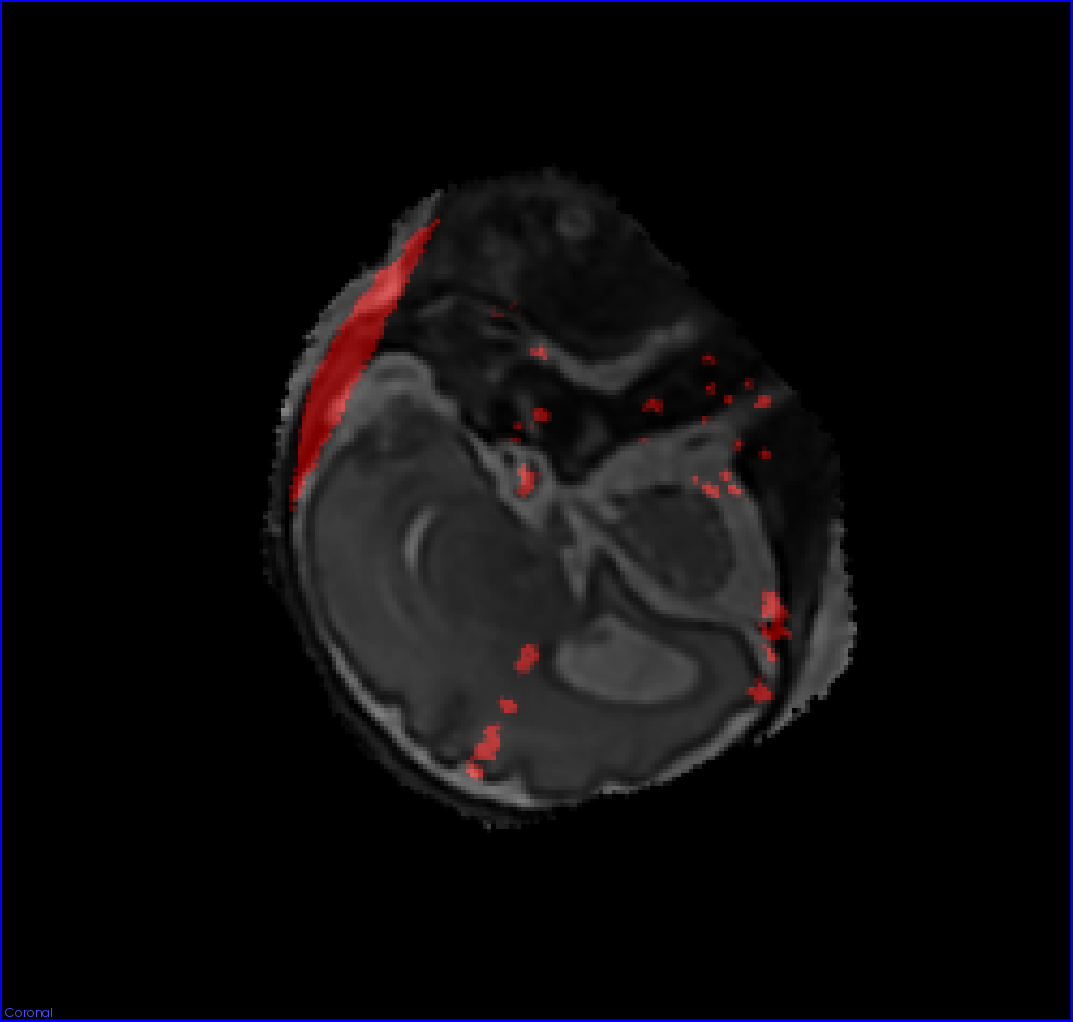
\includegraphics[width=\textwidth]{images/thresholding/results/scan_2d.png}
    \caption{Scan in 2D}
    \label{fig:thresholdingresultsscan2d}
  \end{subfigure}%
  ~ %add desired spacing between images, e. g. ~, \quad, \qquad, \hfill etc.
    %(or a blank line to force the subfigure onto a new line)
  \begin{subfigure}[b]{0.32\textwidth}
    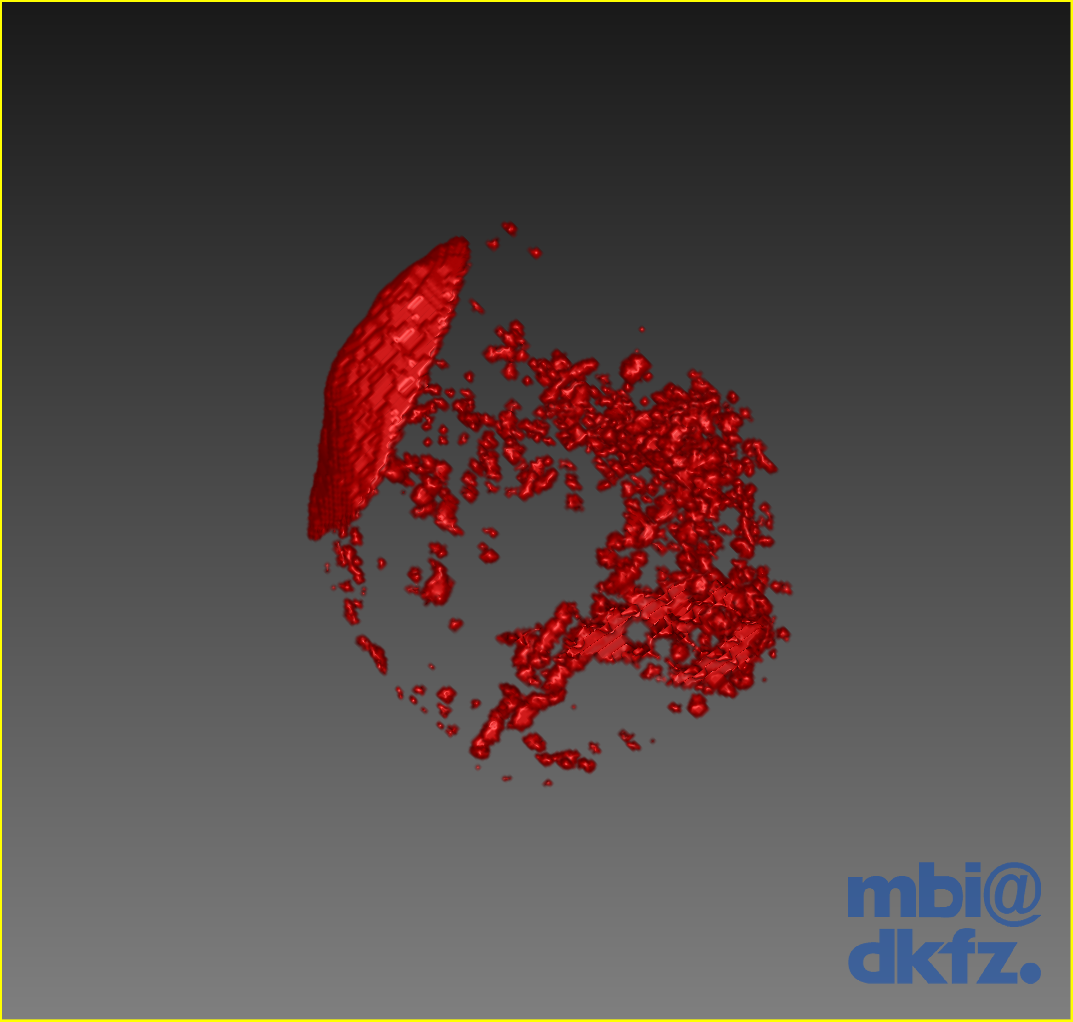
\includegraphics[width=\textwidth]{images/thresholding/results/scan_3d.png}
    \caption{Scan in 3D}
    \label{fig:thresholdingresultsscan3d}
  \end{subfigure}
  % \caption{Opacity Transfer Functions. Opacity of 0 is transparent, 1 is opaque.}\label{fig:thresholdingvariation1problem}
\end{figure}

\newpage
\section{Uncertainty Surface}\label{section:uncertaintysurface}
The idea behind the uncertainty surface is to project the uncertainty (a 3D volume) onto a surface (effectively 2D) to give an overview of the uncertainty hotspots. Two versions have been implemented; the first maps the uncertainty to a sphere and the second maps the uncertainty to a surface representation of the organ being scanned. The uncertainty sphere is a generic visualization that can be applied to any scan, whereas the second requires a surface representation of the organ in question.

Two ways of mapping the uncertainty to the surfaces have been trialled. Originally the uncertainty was mapped to a texture which can then be rendered on a surface model. This worked fairly well for the sphere and figure \ref{fig:uncertaintytexture} shows an example texture that was generated. Each pixel position in the texture (x, y) is first translated to spherical coordinates (\theta, \phi). This can then be converted using trigonometry to a point (x', y', z') on a sphere of unit radius. The uncertainty at pixel (x, y) is then calculated by taking the average uncertainty from the center to the edge travelling in direction (x', y', z').

This technique, however does not translate as well when it comes to mapping the uncertainty onto a generic surface and so an alternative had to be found. As it turned out it is possible to store a scalar value with every point on a surface in MITK and so instead of going via a texture it is possible to store the uncertainty at each point directly.

 This allows both the sphere and generic surface to use the same technique; for each point (on the sphere/surface) a ray is fired into the uncertainty volume to accumulate the uncertainty (see volume rendering section \ref{background:volumerendering}) and the result is mapped to a colour.

\subsection*{Implementation - Sphere}

Firstly a surface representation of a sphere is generated - the resolution of this model can be changed to alter the number of points used to approximate the sphere.

Then each point on the sphere is registered to a start point to begin sampling in the volume (volume intersection in figure). The normal of the point on the sphere is then used as a direction to sample in. The start of the genuine uncertainty is then found by following the sampling direction until the value is not background (uncertainty intersection in figure). Figure \ref{fig:surface_sampling_example} illustrates this process.

\begin{figure}[H]
  \centering
  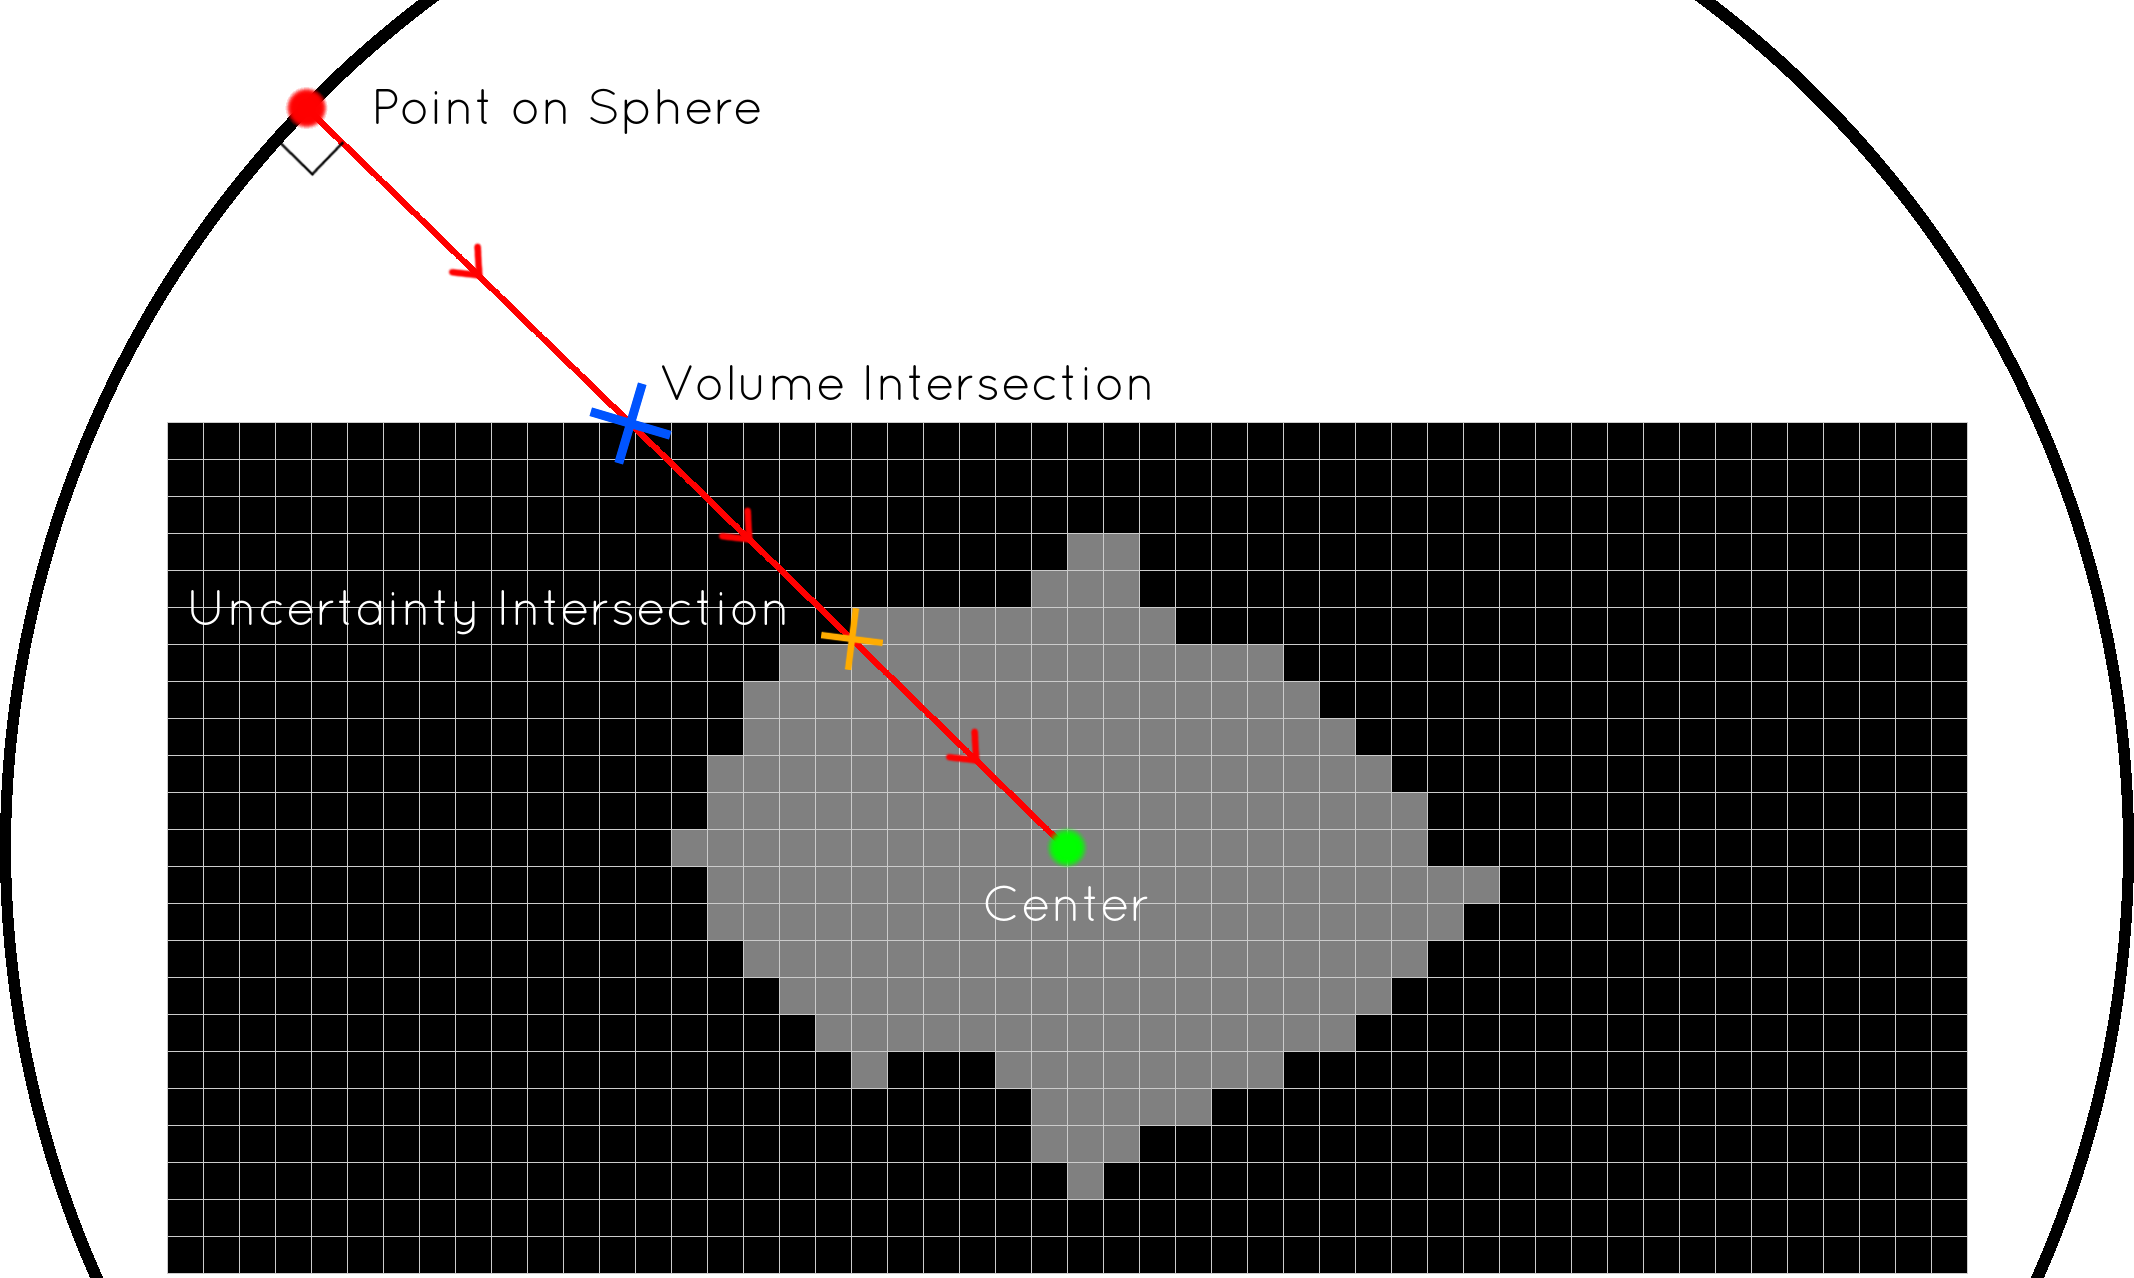
\includegraphics[width=\textwidth]{images/surface/sampling_example.png}
  \caption{Sampling Overview}\label{fig:surface_sampling_example}
\end{figure}

A tortoise and hare algorithm is then used to be able to vary how far into the volume the sampling goes. The tortoise moves through the uncertainty accumulating samples whilst the hare shoots off trying to find the edge. When the hare does find the edge the sampling stops. If the hare travels at the same speed as the tortoise then the entire object is sampled, if it travels at twice the speed of the tortoise then the sampling stops half the way through and so on. This is illustrated in figure \ref{fig:tortoiseandhareexample}.

\begin{figure}[H]
  \centering
  \begin{subfigure}[b]{0.32\textwidth}
    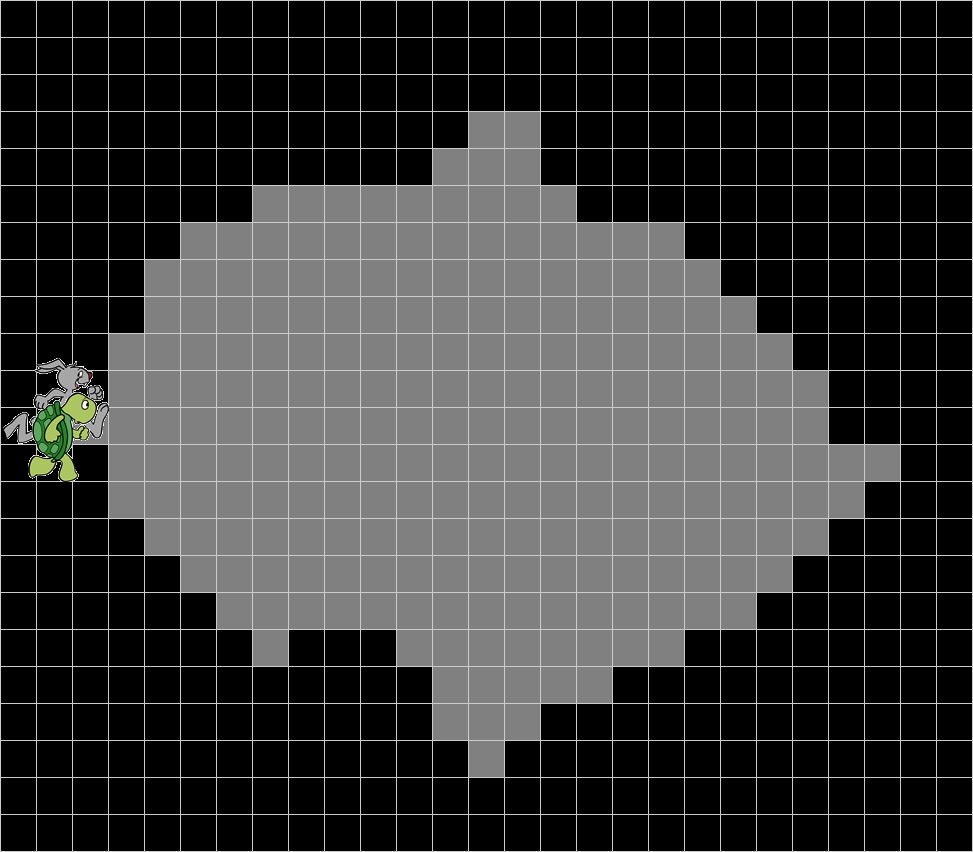
\includegraphics[width=\textwidth]{images/surface/tortoise_and_hare_1.png}
    \caption{Start}
    \label{fig:tortoiseandhare1}
  \end{subfigure}%
  ~ %add desired spacing between images, e. g. ~, \quad, \qquad, \hfill etc.
    %(or a blank line to force the subfigure onto a new line)
  \begin{subfigure}[b]{0.32\textwidth}
    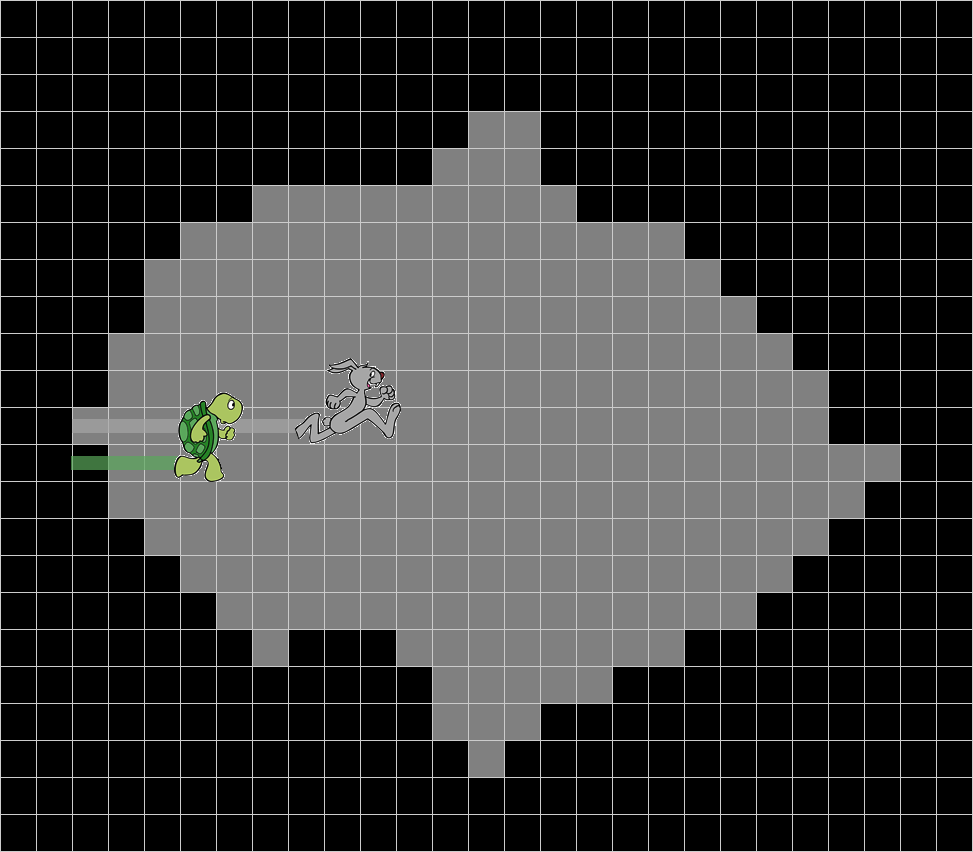
\includegraphics[width=\textwidth]{images/surface/tortoise_and_hare_2.png}
    \caption{...}
    \label{fig:tortoiseandhare2}
  \end{subfigure}%
  ~ %add desired spacing between images, e. g. ~, \quad, \qquad, \hfill etc.
    %(or a blank line to force the subfigure onto a new line)
  \begin{subfigure}[b]{0.32\textwidth}
    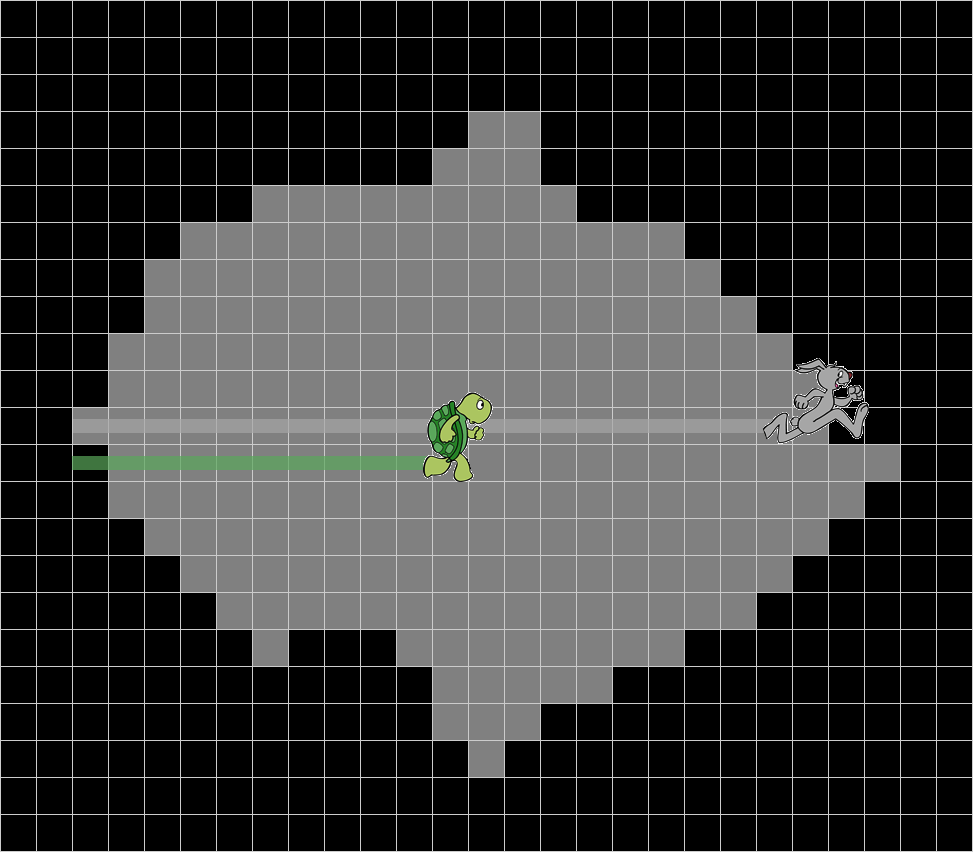
\includegraphics[width=\textwidth]{images/surface/tortoise_and_hare_3.png}
    \caption{End}
    \label{fig:tortoiseandhare3}  
  \end{subfigure}
  \caption{Illustration of Tortoise and Hare Algorithm}\label{fig:tortoiseandhareexample}
\end{figure}

The accumulation that the tortoise does can also be customized. By default it will take the average of all of the samples it takes, but the best value and also the worst value along the ray can be extracted.

Once all of the points have been computed some scaling can be implemented to improve the contrast of the visualization. In many cases the average uncertainty will be roughly the same everywhere and if the range (0-1) is mapped to the entire colour range the values end up looking idential; to fix this the outputted colour range can be linearly mapped to make better use of the colours available.

\subsection*{Implementation - Surface}

To map to a different surface model the procedure is largely the same. Again the first step is to generate the surface representation. Currently this is done using the mask supplied in the reconstruction step - applying surface extraction and mesh decimation (see section \ref{background:surfaceextraction}) to create a rough surface representation.

The registration step in this case is trivial as the mask uses the same coordinate system as the uncertainty volume. The normal at the surface can then be used, as before, and scaling similarly applied.

\newpage
\subsection*{Results}
Scaling was found to significantly increase the contrast of the visualization. The legend shows the scaling applied in each case.

\begin{figure}[H]
  \centering
  \begin{subfigure}[b]{0.25\textwidth}
    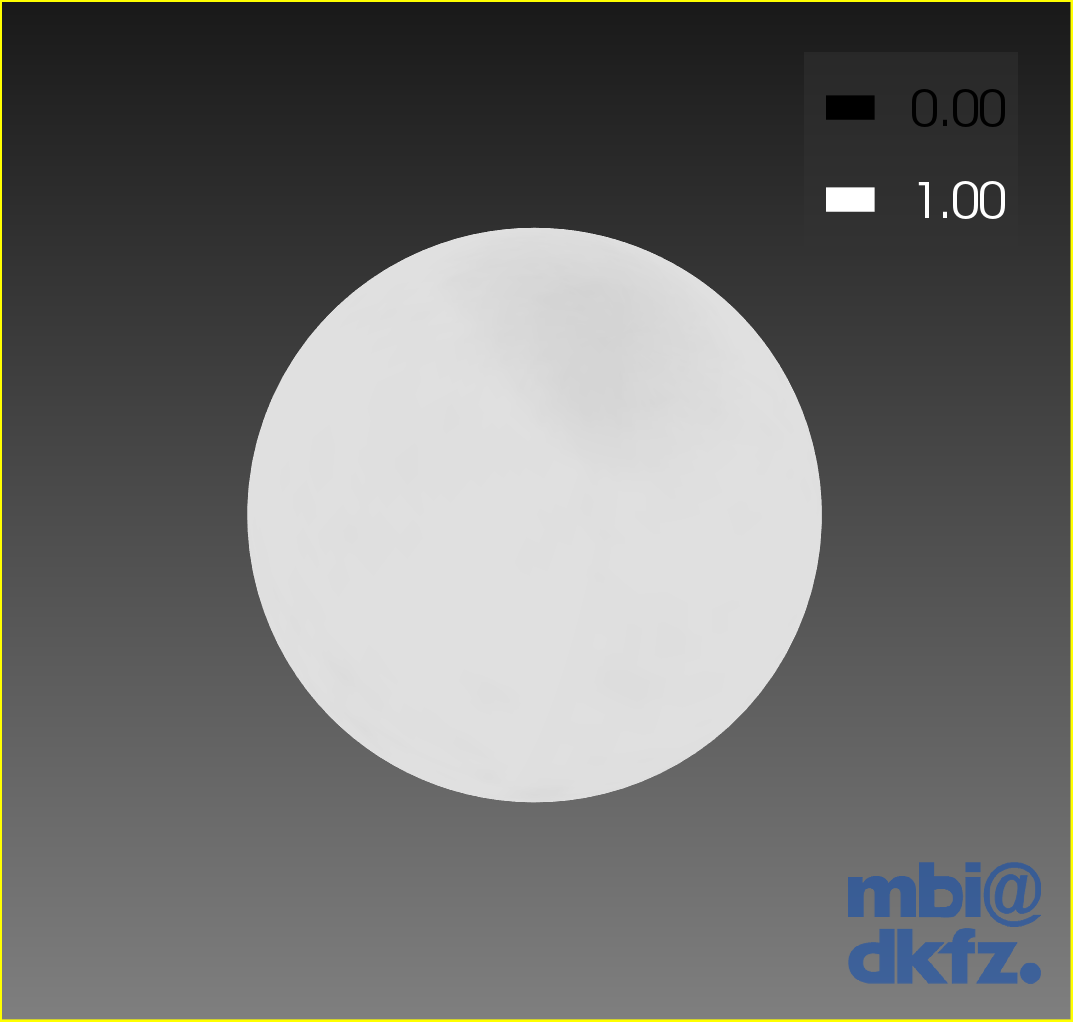
\includegraphics[width=\textwidth]{images/surface/sphere_no_scaling.png}
    \caption*{Sphere\\(No Scaling)}
    \label{fig:surfacespherenoscaling}
  \end{subfigure}%
    %add desired spacing between images, e. g. ~, \quad, \qquad, \hfill etc.
    %(or a blank line to force the subfigure onto a new line)
  \begin{subfigure}[b]{0.25\textwidth}
    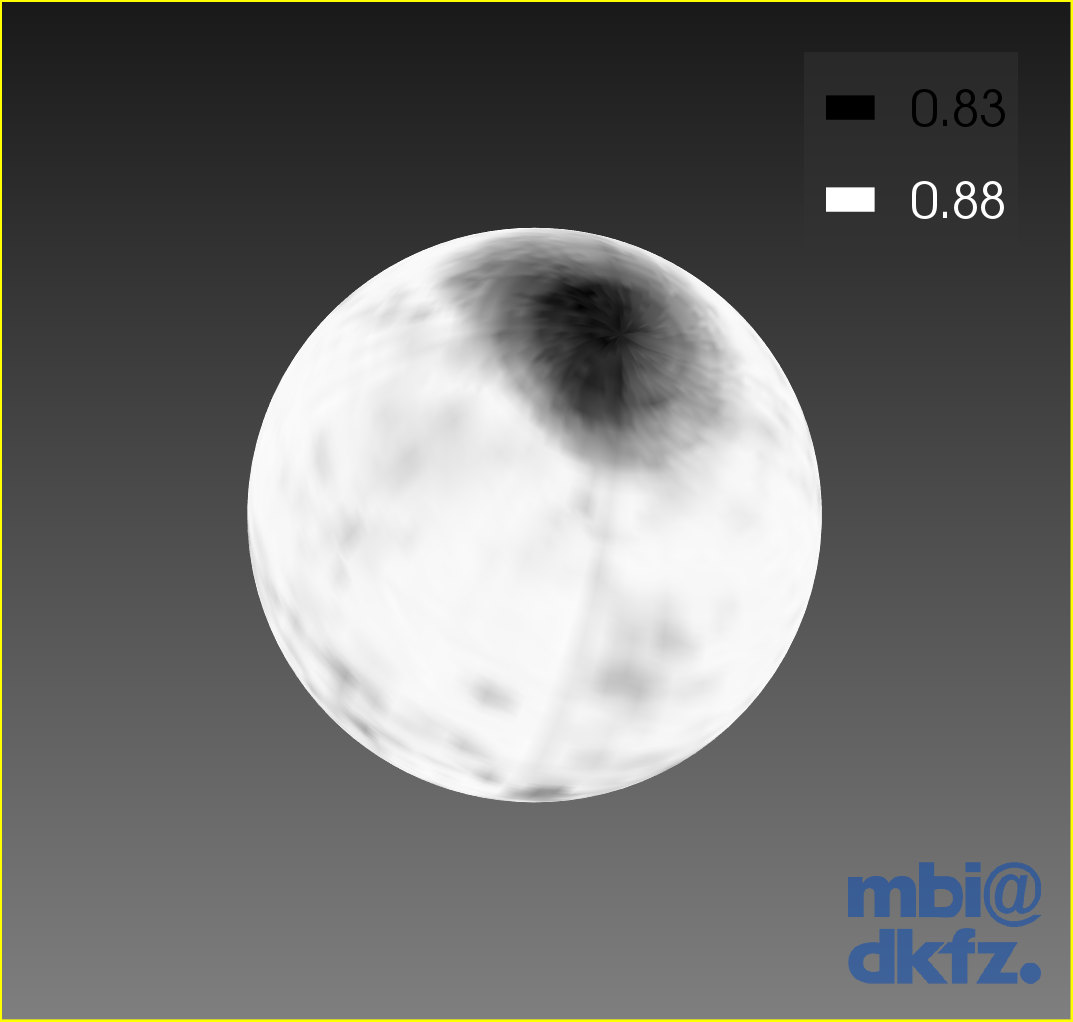
\includegraphics[width=\textwidth]{images/surface/sphere_scaling.png}
    \caption*{Sphere\\(Linear)}
    \label{fig:surfacespherescaling}
  \end{subfigure}%
    %add desired spacing between images, e. g. ~, \quad, \qquad, \hfill etc.
    %(or a blank line to force the subfigure onto a new line)
  \begin{subfigure}[b]{0.25\textwidth}
    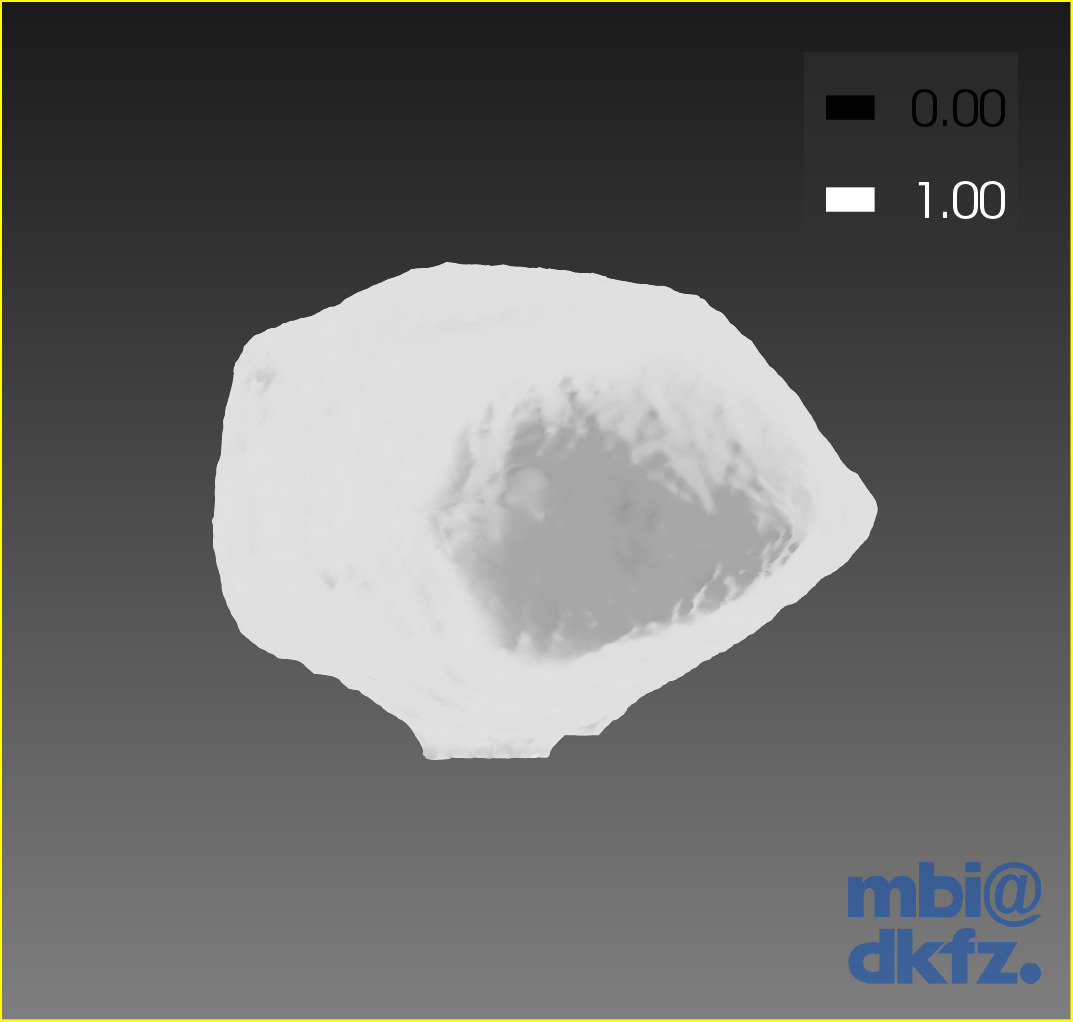
\includegraphics[width=\textwidth]{images/surface/surface_no_scaling.png}
    \caption*{Surface\\(No Scaling)}
    \label{fig:surfacesurfacenoscaling}
  \end{subfigure}%
    %add desired spacing between images, e. g. ~, \quad, \qquad, \hfill etc.
    %(or a blank line to force the subfigure onto a new line)
  \begin{subfigure}[b]{0.25\textwidth}
    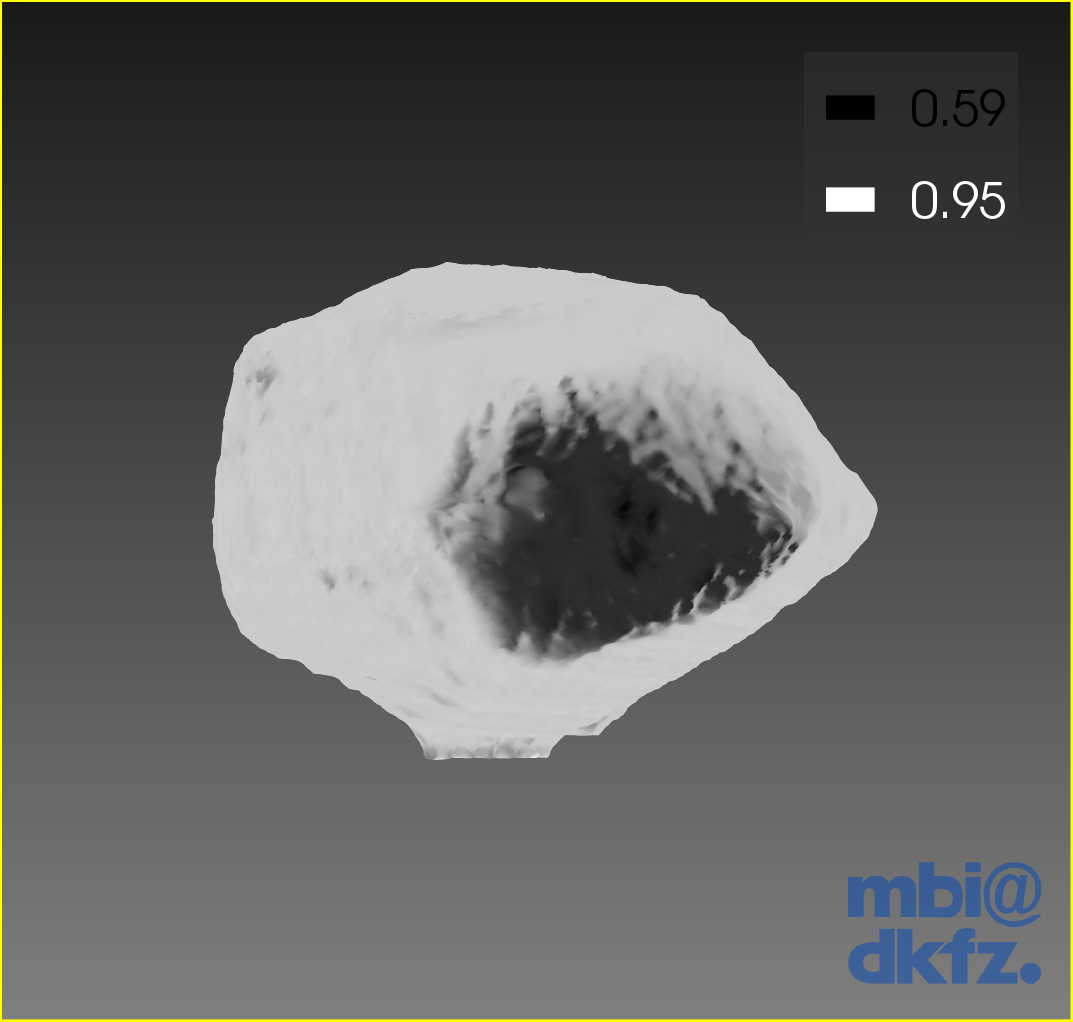
\includegraphics[width=\textwidth]{images/surface/surface_scaling.png}
    \caption*{Sphere\\(Linear)}
    \label{fig:surfacesurfacescaling}
  \end{subfigure}
  \caption{The effect of linear mapping.}\label{fig:surfacescaling}
\end{figure}

The surface representation difficult to interpret by looking at a single image in a report. Figure \ref{fig:surface180} illustrates various angles. In practice all of these visualizations can be rotated and zoomed.

\begin{figure}[h]
  \centering
  \begin{subfigure}[b]{0.20\textwidth}
    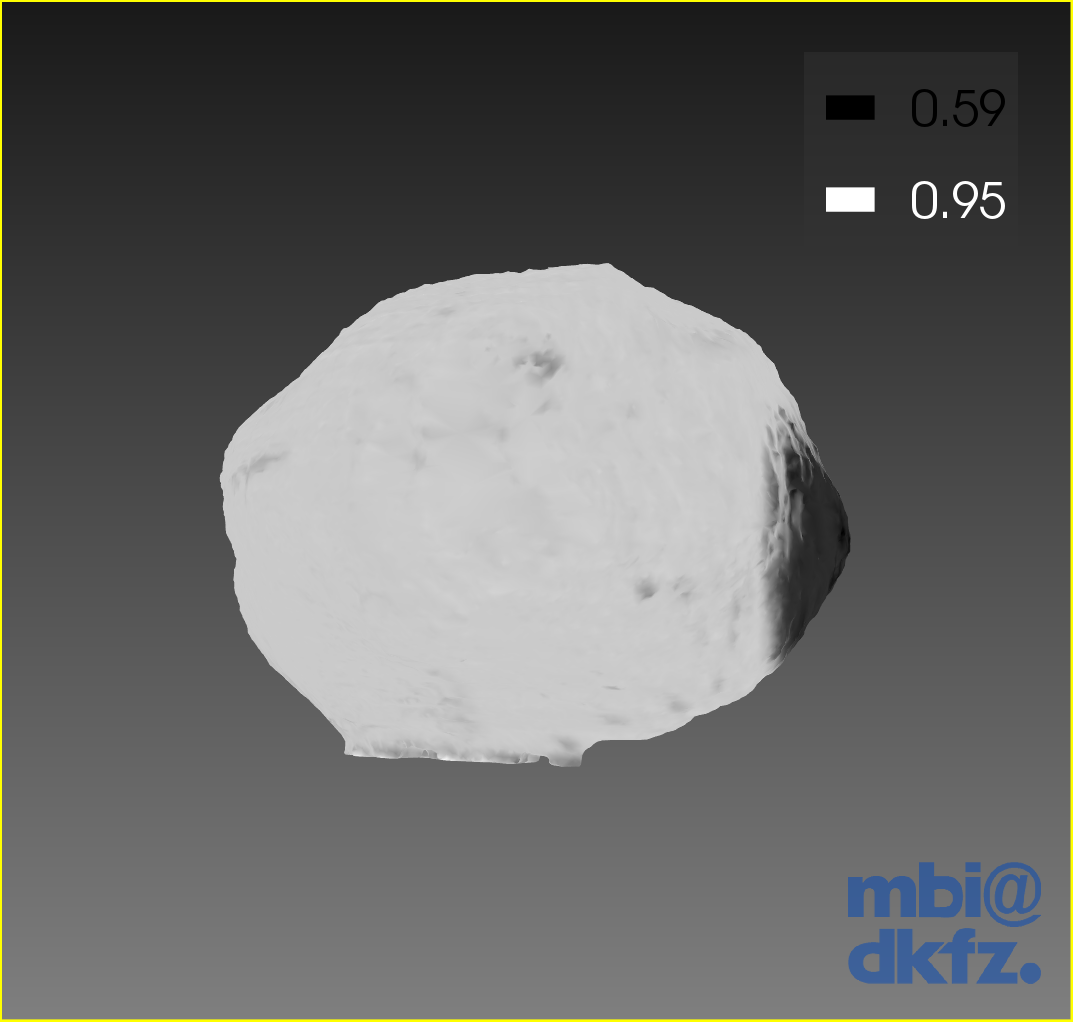
\includegraphics[width=\textwidth]{images/surface/surface_180_1.png}
    \caption*{Left}
    \label{fig:erosion0}
  \end{subfigure}%
    %add desired spacing between images, e. g. ~, \quad, \qquad, \hfill etc.
    %(or a blank line to force the subfigure onto a new line)
  \begin{subfigure}[b]{0.20\textwidth}
    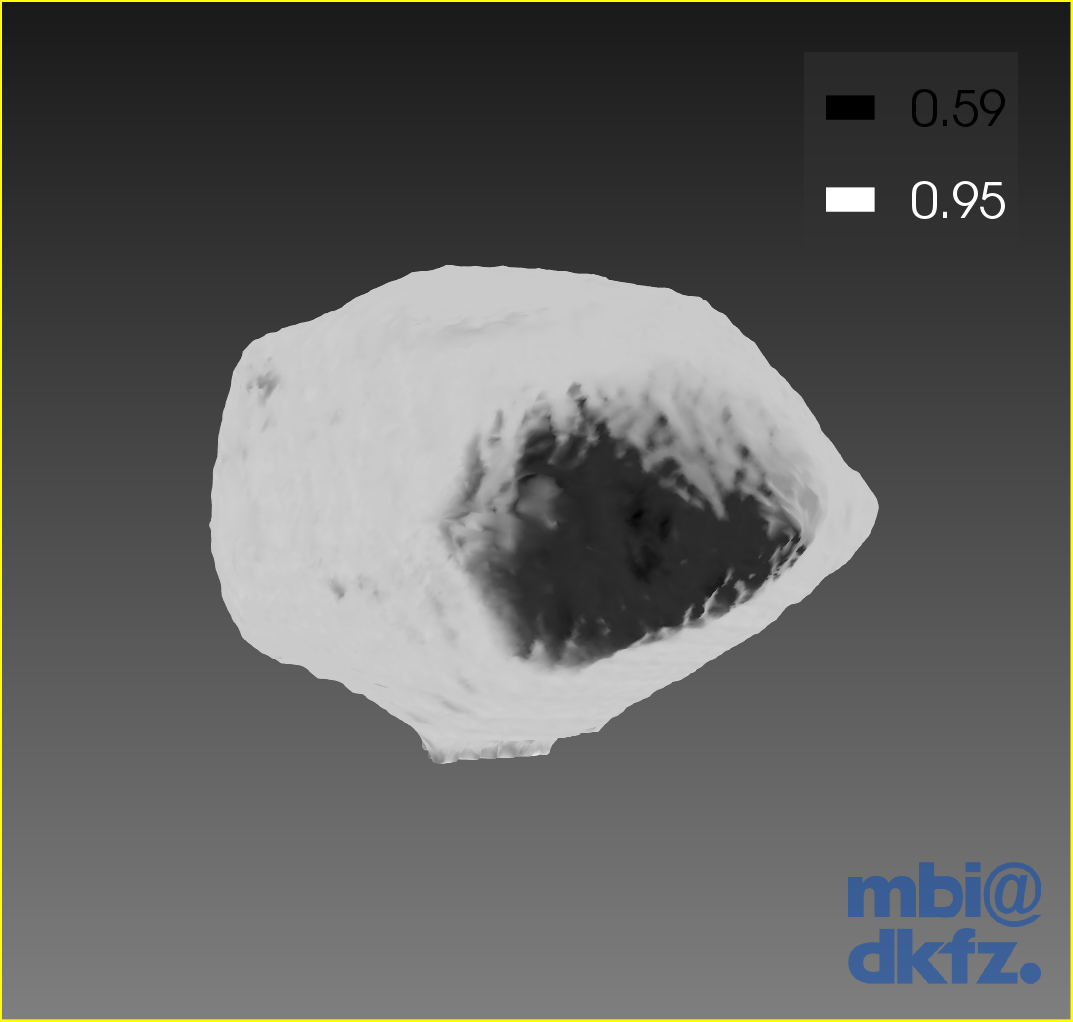
\includegraphics[width=\textwidth]{images/surface/surface_180_2.png}
    \caption*{Front Left}
    \label{fig:erosion1}
  \end{subfigure}%
    %add desired spacing between images, e. g. ~, \quad, \qquad, \hfill etc.
    %(or a blank line to force the subfigure onto a new line)
  \begin{subfigure}[b]{0.20\textwidth}
    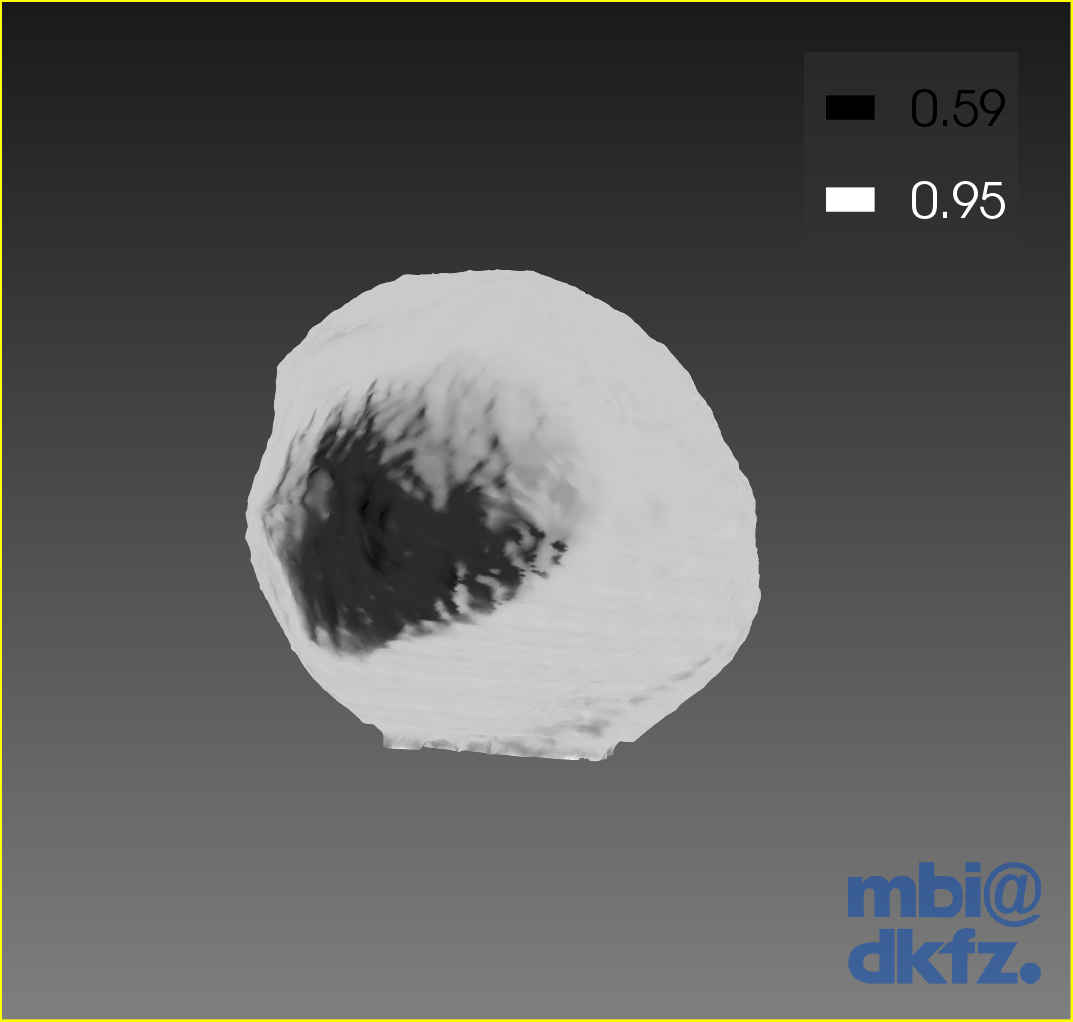
\includegraphics[width=\textwidth]{images/surface/surface_180_3.png}
    \caption*{Front}
    \label{fig:erosion2}
  \end{subfigure}%
    %add desired spacing between images, e. g. ~, \quad, \qquad, \hfill etc.
    %(or a blank line to force the subfigure onto a new line)
  \begin{subfigure}[b]{0.20\textwidth}
    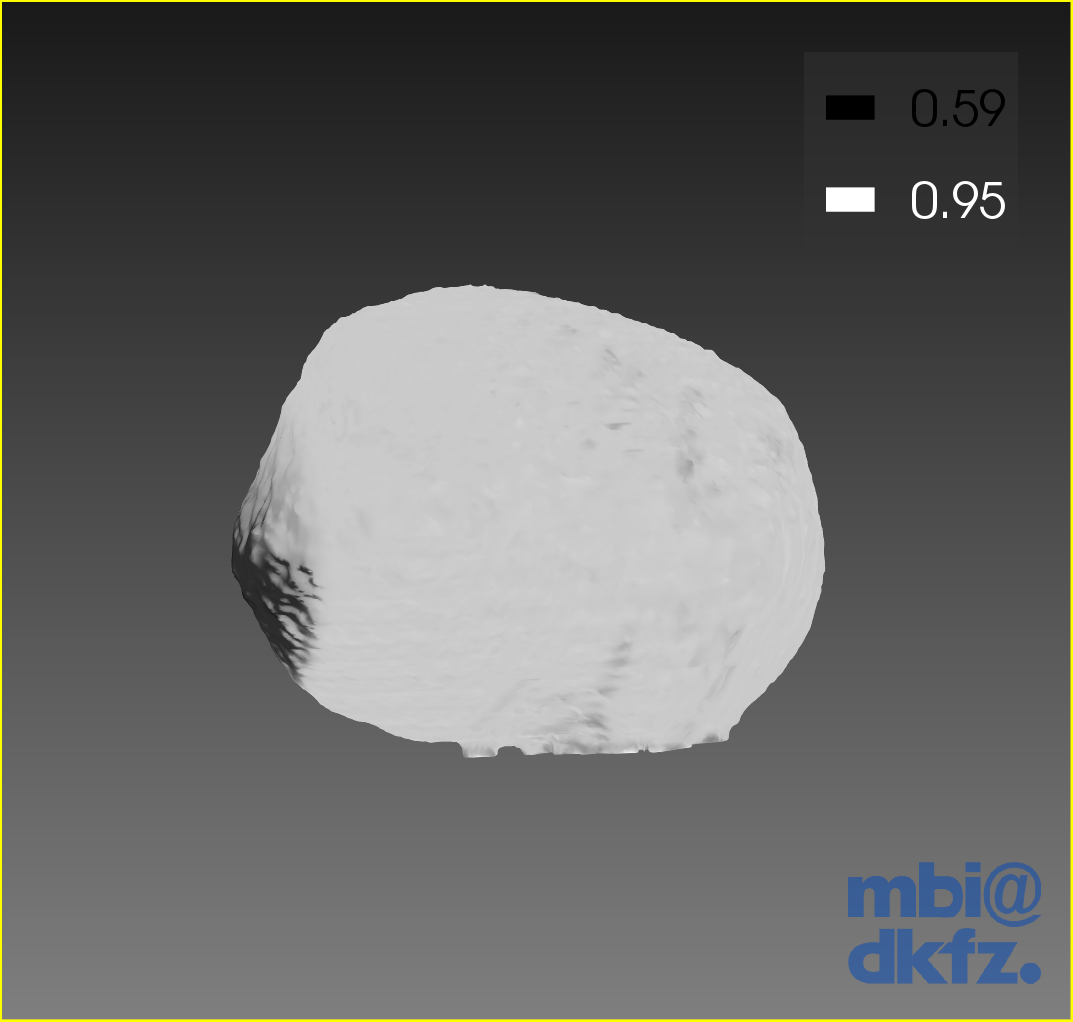
\includegraphics[width=\textwidth]{images/surface/surface_180_4.png}
    \caption*{Front Right}
    \label{fig:erosion3}
  \end{subfigure}%
    %add desired spacing between images, e. g. ~, \quad, \qquad, \hfill etc.
    %(or a blank line to force the subfigure onto a new line)
  \begin{subfigure}[b]{0.20\textwidth}
    \includegraphics[width=\textwidth]{images/surface/surface_180_5.png}
    \caption*{Right}
    \label{fig:erosion3}
  \end{subfigure}
  \caption{Brain surface viewed from different directions.}\label{fig:surface180}
\end{figure}

The default behaviour of taking the average uncertainty along the ray does a good job of bringing out the uncertainty but switching to the worst brings severe values that would otherwise be outweighed by good values to the surface. Switching to the best value isolates only truly terrible areas.

\begin{figure}[H]
  \centering
  \begin{subfigure}[b]{0.32\textwidth}
    \includegraphics[width=\textwidth]{images/surface/sphere_average.png}
    \caption{Average}
    \label{fig:sphereaverage}
  \end{subfigure}%
  ~ %add desired spacing between images, e. g. ~, \quad, \qquad, \hfill etc.
    %(or a blank line to force the subfigure onto a new line)
  \begin{subfigure}[b]{0.32\textwidth}
    \includegraphics[width=\textwidth]{images/surface/sphere_worst.png}
    \caption{Worst}
    \label{fig:sphereworst}
  \end{subfigure}%
  ~ %add desired spacing between images, e. g. ~, \quad, \qquad, \hfill etc.
    %(or a blank line to force the subfigure onto a new line)
  \begin{subfigure}[b]{0.32\textwidth}
    \includegraphics[width=\textwidth]{images/surface/sphere_best.png}
    \caption{Best}
    \label{fig:spherebest}  
  \end{subfigure}
  ~ %add desired spacing between images, e. g. ~, \quad, \qquad, \hfill etc.
    %(or a blank line to force the subfigure onto a new line)  
  \begin{subfigure}[b]{0.32\textwidth}
    \includegraphics[width=\textwidth]{images/surface/surface_average.png}
    \caption{Average}
    \label{fig:surfaceaverage}
  \end{subfigure}%
  ~ %add desired spacing between images, e. g. ~, \quad, \qquad, \hfill etc.
    %(or a blank line to force the subfigure onto a new line)
  \begin{subfigure}[b]{0.32\textwidth}
    \includegraphics[width=\textwidth]{images/surface/surface_worst.png}
    \caption{Worst}
    \label{fig:surfaceworst}
  \end{subfigure}%
  ~ %add desired spacing between images, e. g. ~, \quad, \qquad, \hfill etc.
    %(or a blank line to force the subfigure onto a new line)
  \begin{subfigure}[b]{0.32\textwidth}
    \includegraphics[width=\textwidth]{images/surface/surface_best.png}
    \caption{Best}
    \label{fig:surfacebest}  
  \end{subfigure}  
  \caption{Comparison of Average/Best/Worst sampling.}\label{fig:surfaceaccumulator}
\end{figure}

The sample distance determines how far into the volume samples go. Currently there are two options available - half and full. These options are less applicable to the sphere as if it is set to full then opposite sides of the sphere give identical values. When applied to the surface the use of this option very much depends on the area of the body that is being scanned. The brain is a large, and for the most part (ignoring folds particularly) convex; in this respect it is similar to the sphere and the effect of sampling all the way through is much the same (see figure \ref{fig:surfacesampledistance}). You can notice that the average uncertainty gets better with full sampling as there are more good points to outweigh the bad.

\begin{figure}[H]
  \centering
  \begin{subfigure}[b]{0.5\textwidth}
    \includegraphics[width=\textwidth]{images/surface/surface_half.png}
    \caption{Half}
    \label{fig:surfacehalf}
  \end{subfigure}%
  ~ %add desired spacing between images, e. g. ~, \quad, \qquad, \hfill etc.
    %(or a blank line to force the subfigure onto a new line)
  \begin{subfigure}[b]{0.5\textwidth}
    \includegraphics[width=\textwidth]{images/surface/surface_full.png}
    \caption{Full}
    \label{fig:surfacefull}
  \end{subfigure}
  \caption{Comparing half and full distance sampling.}\label{fig:surfacesampledistance}
\end{figure}

Where this parameter may be more useful however is when dealing with smaller, more intricate objects, such as arteries. It would allow the uncertainty the entire cross section to be mapped to the surface which would give an overview of the uncertainty in that section at a glance, rather than having to rotate around it to get the full picture.

\newpage
\section{Next Scan Plane}\label{section:nextscanplane}
The idea behind this visualization is based on some previous research\cite{uncertaintysvd} on finding the optimum place to scan next given the current uncertainty. With this knowledge the scanning process can continually target areas of uncertainty to optimize the quality of the scan.

This visualization is designed to communicate this next best scan to the radiographer in a way that gives them some context as to why this is in some sense optimal.

The main obstacle that prevents this being integrated into MRI scanners currently is the fact that the reconstruction code takes far too long to run during a scan, which generally last no longer than 45-60 minutes.

\subsection*{Implementation}
The technique, based on SVD, takes in a set of points, and finds the optimal direction to scan in. The implementation lets the user determine the set of points given to the algorithm by specifying a threshold of uncertainty. Before generating the next scan the threshold is first visualized, using the thresholding visualization (section \ref{section:thresholding}). Then the SVD implementation from the VNL numerics library is then used to produce the scan direction and center point.

The resulting scan is then visualized as a circle which shows the center of the scan, and a cylinder which shows the direction of the scan. The reason that the scan is shown as a circle is because the technique only determines the scan direction (z-axis/slice direction) and not the x and y axes.

The next scan plane can be overlayed on both the thresholded uncertainty as well as a volume rendering of the original scan.

\subsection*{Results}

Figure \ref{fig:nextscanplane} illustrates the process the user goes through.

\begin{figure}[H]
  \centering
  \begin{subfigure}[b]{0.32\textwidth}
    \includegraphics[width=\textwidth]{images/next_scan_plane/next_scan_plane_threshold.png}
    \caption{Target Uncertainty}
    \label{fig:nextscanplanethreshold}
  \end{subfigure}%
  ~ %add desired spacing between images, e. g. ~, \quad, \qquad, \hfill etc.
    %(or a blank line to force the subfigure onto a new line)
  \begin{subfigure}[b]{0.32\textwidth}
    \includegraphics[width=\textwidth]{images/next_scan_plane/next_scan_plane_1.png}
    \caption{Next Scan Plane}
    \label{fig:nextscanplane1}
  \end{subfigure}%
  ~ %add desired spacing between images, e. g. ~, \quad, \qquad, \hfill etc.
    %(or a blank line to force the subfigure onto a new line)
  \begin{subfigure}[b]{0.32\textwidth}
    \includegraphics[width=\textwidth]{images/next_scan_plane/next_scan_plane_2.png}
    \caption{With Scan}
    \label{fig:nextscanplane2}  
  \end{subfigure}
  \caption{Comparison of Average/Best/Worst sampling.}\label{fig:nextscanplane}
\end{figure}

Figure \ref{fig:nextscanplanetests} shows the next scan planes for the test uncertainties. The sphere and sphere in corner can be scanned from any direction as they have infinitely many lines of symettry. The cube is scanned such that the maximum number of slices hits it. The random volume, similar to the sphere, is also best scanned from one of the three main axes.

\begin{figure}[H]
  \centering
  \begin{subfigure}[b]{0.5\textwidth}
    \includegraphics[width=\textwidth]{images/next_scan_plane/sphere.png}
    \caption{Sphere}
    \label{fig:nextscanplanesphere}
  \end{subfigure}%
  ~ %add desired spacing between images, e. g. ~, \quad, \qquad, \hfill etc.
    %(or a blank line to force the subfigure onto a new line)
  \begin{subfigure}[b]{0.5\textwidth}
    \includegraphics[width=\textwidth]{images/next_scan_plane/sphere_in_corner.png}
    \caption{Sphere in Corner}
    \label{fig:nextscanplanespherecorner}
  \end{subfigure}
  ~%add desired spacing between images, e. g. ~, \quad, \qquad, \hfill etc.
    %(or a blank line to force the subfigure onto a new line)
  \begin{subfigure}[b]{0.5\textwidth}
    \includegraphics[width=\textwidth]{images/next_scan_plane/cube.png}
    \caption{Cube}
    \label{fig:nextscanplanecube}  
  \end{subfigure}%
  ~ %add desired spacing between images, e. g. ~, \quad, \qquad, \hfill etc.
    %(or a blank line to force the subfigure onto a new line)
  \begin{subfigure}[b]{0.5\textwidth}
    \includegraphics[width=\textwidth]{images/next_scan_plane/random.png}
    \caption{Random}
    \label{fig:nextscanplanerandom}  
  \end{subfigure}  
  \caption{Next scan planes for the test uncertainties.}\label{fig:nextscanplanetests}
\end{figure}

The next scan plane can also be displayed in the 2D view (figure \ref{fig:nextscanplane2d}).

\begin{figure}[H]
  \centering
  \begin{subfigure}[b]{0.3\textwidth}
    \includegraphics[width=\textwidth]{images/next_scan_plane/axial.png}
    \caption*{Axial}
    \label{fig:nextscanplaneaxial}
  \end{subfigure}%
  ~ %add desired spacing between images, e. g. ~, \quad, \qquad, \hfill etc.
    %(or a blank line to force the subfigure onto a new line)
  \begin{subfigure}[b]{0.3\textwidth}
    \includegraphics[width=\textwidth]{images/next_scan_plane/coronal.png}
    \caption*{Coronal}
    \label{fig:nextscanplanecoronal}
  \end{subfigure}%
  ~%add desired spacing between images, e. g. ~, \quad, \qquad, \hfill etc.
    %(or a blank line to force the subfigure onto a new line)
  \begin{subfigure}[b]{0.3\textwidth}
    \includegraphics[width=\textwidth]{images/next_scan_plane/sagittal.png}
    \caption*{Sagittal}
    \label{fig:nextscanplanesagittal}
  \end{subfigure}
  \caption{Next Scan Plane in 2D}\label{fig:nextscanplane2d}
\end{figure}